% Options for packages loaded elsewhere
\PassOptionsToPackage{unicode}{hyperref}
\PassOptionsToPackage{hyphens}{url}
%
\documentclass[
  english,
  doc,12pt,twoside,floatsintext]{apa7}
\usepackage{amsmath,amssymb}
\usepackage{lmodern}
\usepackage{ifxetex,ifluatex}
\ifnum 0\ifxetex 1\fi\ifluatex 1\fi=0 % if pdftex
  \usepackage[T1]{fontenc}
  \usepackage[utf8]{inputenc}
  \usepackage{textcomp} % provide euro and other symbols
\else % if luatex or xetex
  \usepackage{unicode-math}
  \defaultfontfeatures{Scale=MatchLowercase}
  \defaultfontfeatures[\rmfamily]{Ligatures=TeX,Scale=1}
  \setmainfont[]{Times New Roman}
\fi
% Use upquote if available, for straight quotes in verbatim environments
\IfFileExists{upquote.sty}{\usepackage{upquote}}{}
\IfFileExists{microtype.sty}{% use microtype if available
  \usepackage[]{microtype}
  \UseMicrotypeSet[protrusion]{basicmath} % disable protrusion for tt fonts
}{}
\makeatletter
\@ifundefined{KOMAClassName}{% if non-KOMA class
  \IfFileExists{parskip.sty}{%
    \usepackage{parskip}
  }{% else
    \setlength{\parindent}{0pt}
    \setlength{\parskip}{6pt plus 2pt minus 1pt}}
}{% if KOMA class
  \KOMAoptions{parskip=half}}
\makeatother
\usepackage{xcolor}
\IfFileExists{xurl.sty}{\usepackage{xurl}}{} % add URL line breaks if available
\IfFileExists{bookmark.sty}{\usepackage{bookmark}}{\usepackage{hyperref}}
\hypersetup{
  pdftitle={This page and the next page should be removed},
  pdflang={en-EN},
  hidelinks,
  pdfcreator={LaTeX via pandoc}}
\urlstyle{same} % disable monospaced font for URLs
\usepackage{graphicx}
\makeatletter
\def\maxwidth{\ifdim\Gin@nat@width>\linewidth\linewidth\else\Gin@nat@width\fi}
\def\maxheight{\ifdim\Gin@nat@height>\textheight\textheight\else\Gin@nat@height\fi}
\makeatother
% Scale images if necessary, so that they will not overflow the page
% margins by default, and it is still possible to overwrite the defaults
% using explicit options in \includegraphics[width, height, ...]{}
\setkeys{Gin}{width=\maxwidth,height=\maxheight,keepaspectratio}
% Set default figure placement to htbp
\makeatletter
\def\fps@figure{htbp}
\makeatother
\setlength{\emergencystretch}{3em} % prevent overfull lines
\providecommand{\tightlist}{%
  \setlength{\itemsep}{0pt}\setlength{\parskip}{0pt}}
\setcounter{secnumdepth}{5}
% Make \paragraph and \subparagraph free-standing
\ifx\paragraph\undefined\else
  \let\oldparagraph\paragraph
  \renewcommand{\paragraph}[1]{\oldparagraph{#1}\mbox{}}
\fi
\ifx\subparagraph\undefined\else
  \let\oldsubparagraph\subparagraph
  \renewcommand{\subparagraph}[1]{\oldsubparagraph{#1}\mbox{}}
\fi
% Manuscript styling
\usepackage{upgreek}
\captionsetup{font=singlespacing,justification=justified}

% Table formatting
\usepackage{longtable}
\usepackage{lscape}
% \usepackage[counterclockwise]{rotating}   % Landscape page setup for large tables
\usepackage{multirow}		% Table styling
\usepackage{tabularx}		% Control Column width
\usepackage[flushleft]{threeparttable}	% Allows for three part tables with a specified notes section
\usepackage{threeparttablex}            % Lets threeparttable work with longtable

% Create new environments so endfloat can handle them
% \newenvironment{ltable}
%   {\begin{landscape}\begin{center}\begin{threeparttable}}
%   {\end{threeparttable}\end{center}\end{landscape}}
\newenvironment{lltable}{\begin{landscape}\begin{center}\begin{ThreePartTable}}{\end{ThreePartTable}\end{center}\end{landscape}}

% Enables adjusting longtable caption width to table width
% Solution found at http://golatex.de/longtable-mit-caption-so-breit-wie-die-tabelle-t15767.html
\makeatletter
\newcommand\LastLTentrywidth{1em}
\newlength\longtablewidth
\setlength{\longtablewidth}{1in}
\newcommand{\getlongtablewidth}{\begingroup \ifcsname LT@\roman{LT@tables}\endcsname \global\longtablewidth=0pt \renewcommand{\LT@entry}[2]{\global\advance\longtablewidth by ##2\relax\gdef\LastLTentrywidth{##2}}\@nameuse{LT@\roman{LT@tables}} \fi \endgroup}

% \setlength{\parindent}{0.5in}
% \setlength{\parskip}{0pt plus 0pt minus 0pt}

% Overwrite redefinition of paragraph and subparagraph by the default LaTeX template
% See https://github.com/crsh/papaja/issues/292
\makeatletter
\renewcommand{\paragraph}{\@startsection{paragraph}{4}{\parindent}%
  {0\baselineskip \@plus 0.2ex \@minus 0.2ex}%
  {-1em}%
  {\normalfont\normalsize\bfseries\itshape\typesectitle}}

\renewcommand{\subparagraph}[1]{\@startsection{subparagraph}{5}{1em}%
  {0\baselineskip \@plus 0.2ex \@minus 0.2ex}%
  {-\z@\relax}%
  {\normalfont\normalsize\itshape\hspace{\parindent}{#1}\textit{\addperi}}{\relax}}
\makeatother

% \usepackage{etoolbox}
\makeatletter
\patchcmd{\HyOrg@maketitle}
  {\section{\normalfont\normalsize\abstractname}}
  {\section*{\normalfont\normalsize\abstractname}}
  {}{\typeout{Failed to patch abstract.}}
\patchcmd{\HyOrg@maketitle}
  {\section{\protect\normalfont{\@title}}}
  {\section*{\protect\normalfont{\@title}}}
  {}{\typeout{Failed to patch title.}}
\makeatother
\shorttitle{}
\usepackage{csquotes}
\geometry{a4paper,margin=25mm}
\setcounter{tocdepth}{2}
\raggedbottom
\usepackage{ragged2e}
\linespread{1.5}
\fancyhead{}
\fancyheadoffset[RO,LE]{0pt}
\fancyhead[RO,LE]{\thepage}
\fancyhead[RE,LO]{Semantic Knowledge and Unfamiliar Objects}
\renewcommand{\headrulewidth}{0.4pt}
\usepackage{setspace}
\AtBeginEnvironment{tabular}{\doublespacing}
\usepackage{makecell}
\renewcommand{\cellset}{\renewcommand{\arraystretch}{0.7}}
\captionsetup[table]{font={stretch=1.5}}
\captionsetup[figure]{font={stretch=1.5}}
\usepackage[all]{nowidow}
\usepackage[bottom]{footmisc}
\interfootnotelinepenalty=10000
\usepackage[export]{adjustbox}
\ifxetex
  % Load polyglossia as late as possible: uses bidi with RTL langages (e.g. Hebrew, Arabic)
  \usepackage{polyglossia}
  \setmainlanguage[]{english}
\else
  \usepackage[main=english]{babel}
% get rid of language-specific shorthands (see #6817):
\let\LanguageShortHands\languageshorthands
\def\languageshorthands#1{}
\fi
\ifluatex
  \usepackage{selnolig}  % disable illegal ligatures
\fi
\newlength{\cslhangindent}
\setlength{\cslhangindent}{1.5em}
\newlength{\csllabelwidth}
\setlength{\csllabelwidth}{3em}
\newenvironment{CSLReferences}[2] % #1 hanging-ident, #2 entry spacing
 {% don't indent paragraphs
  \setlength{\parindent}{0pt}
  % turn on hanging indent if param 1 is 1
  \ifodd #1 \everypar{\setlength{\hangindent}{\cslhangindent}}\ignorespaces\fi
  % set entry spacing
  \ifnum #2 > 0
  \setlength{\parskip}{#2\baselineskip}
  \fi
 }%
 {}
\usepackage{calc}
\newcommand{\CSLBlock}[1]{#1\hfill\break}
\newcommand{\CSLLeftMargin}[1]{\parbox[t]{\csllabelwidth}{#1}}
\newcommand{\CSLRightInline}[1]{\parbox[t]{\linewidth - \csllabelwidth}{#1}\break}
\newcommand{\CSLIndent}[1]{\hspace{\cslhangindent}#1}

\title{This page and the next page should be removed}
\author{\textsuperscript{}}
\date{}


\affiliation{\vspace{0.5cm}\textsuperscript{} }

\begin{document}
\maketitle

\clearpage

\mbox{}\thispagestyle{empty}\clearpage

\thispagestyle{empty}
\begin{center}
\vspace*{10mm}
\textbf{Event-Related Potentials of the Semantically Informed}\\
\textbf{Perception of Unfamiliar Objects}\\
\vspace*{5mm}
\begin{figure}[h]
\begin{center}

\includegraphics[width=!,totalheight=!,scale=0.25]{master_thesis_files/hu_logo}
\end{center}
\end{figure}
{\setstretch{1.5}
Masterarbeit\\
an der\\
Humboldt-Universität zu Berlin\\
zur Erlangung des akademischen Grades \\
Master of Science (M.Sc.)\\
im Fach Psychologie\\
\vspace*{25mm}
}
\end{center}
\begin{flushleft}
{\setstretch{1.5}
\begin{tabular}{ll}
Vorgelegt von:&\textbf{Alexander Enge}\\
&geb. am 09.11.1996 in Räckelwitz\\
&Matrikelnummer 581331\\
Fachliche Betreuung:&Prof. Dr. Rasha Abdel Rahman (Humboldt-Universität zu Berlin)\\
&Prof. Dr. Franziska Süß (Fachhochschule des Mittelstands)\\
&\\
Berlin, den 26.01.2021&\\
\end{tabular}
}
\end{flushleft}

\clearpage

\mbox{}\thispagestyle{empty}\clearpage

\thispagestyle{empty}

\vspace*{55mm}

\begin{center}\textbf{Acknowledgments}\end{center}

This thesis presents a re-analysis of the data from two experiments that had already been conducted before I joined the Neurocognitive Psychology Lab at Humboldt-Universität zu Berlin. Therefore, it would not have been possible for me to write it without the time and effort that Franziska Süß, Nele Langosch, and Rasha Abdel Rahman have spent conceptualizing and running these experiments, along with the help of all participants, research assistants, and technical staff who contributed to the data collection. I would also like to thank all current members of the lab for their guidance and fruitful discussions on the topics of data analysis and reporting. Valuable feedback on an earlier draft of this thesis was given by Anna Kuhlen, Annika Just, and Garrett Widener. Finally, I am most grateful to my parents, friends, and supervisors: During the journey of writing this thesis, their support has often literally changed my view of the world around me to the better.

\clearpage

\mbox{}\thispagestyle{empty}\clearpage

\thispagestyle{empty}

\vspace*{45mm}

\begin{flushleft}
{\setstretch{1.0}
\tableofcontents
}
\end{flushleft}

\clearpage

\mbox{}\thispagestyle{empty}\clearpage

\setcounter{page}{1}

\hypertarget{abstract}{%
\section*{Abstract}\label{abstract}}
\addcontentsline{toc}{section}{Abstract}

\noindent Does our perception of an object change as soon as we discover what function it serves? This question is relevant not only for our everyday lives, where we may encounter novel tools and gadgets as parts of our dynamic working and private environments; it also pertains to the long-standing debate around the (im)penetrability of perception by higher cognitive capacities. In this experiment, we showed participants (\emph{n} = 24) pictures of 120 unfamiliar objects either together with matching information about their function---leading to semantically informed perception---or together with non-matching information---resulting in naive perception. We measured event-related potentials (ERPs) to investigate at which stages in the visual processing hierarchy these two types of object perception differed from one another. We found that semantically informed as compared to naive perception was associated with larger amplitudes in the N170 component and reduced amplitudes in the N400 component. When the same objects were presented once more (without any information), the N400 effect persisted and we now also observed enlarged amplitudes in the P1 component in response to objects for which semantically informed perception had taken place. We replicated these novel findings in an independent sample (\emph{n} = 24). Consistent with previous work, these results suggest that obtaining semantic information about previously unfamiliar objects alters aspects of their lower-level visual perception (P1 component), higher-level visual perception (e.g., holistic perception; N170 component), and semantic processing (N400 component).

\emph{Keywords:} objects, semantic knowledge, visual perception, event-related potentials

\newpage

\hypertarget{introduction}{%
\section{Introduction}\label{introduction}}

Does our perception of an object change as soon as we discover what function it serves? In this study, we presented participants with unfamiliar objects that were preceded either by matching information about their function, leading to semantically informed perception, or by non-matching information, leading to naive perception. We expected semantically informed perception to differ from naive perception within the object processing hierarchy and we capitalized on the high temporal resolution of event-related potentials (ERPs) to find out at which stage (or stages) this was indeed the case. It allowed us to show for the first time that knowledge about the function of a previously unfamiliar object alters its early cortical processing in the same trial as it is being discovered and within less than 200 ms after the presentation of the object.

The claim that higher-level cognitive capacities such as knowledge or language can modulate lower-level perceptual processes has been the source of a long-running debate. This debate revolves around the question of whether or not our perception of the (visual) world is ``cognitively impenetrable'' (Pylyshyn, 1999) or, in other words, determined solely by the visual input reaching our retina. According to one view, higher-level mental states and functions are not able to penetrate perception and kick in only after lower-level perceptual analysis of the visual input has taken pace (e.g., Firestone \& Scholl, 2016; Fodor, 1983; Pylyshyn, 1999). Visual perception itself is treated as an encapsulated module that processes the retinal input in a feed-forward fashion, progressing from lower areas with smaller receptive field sizes to areas representing increasingly complex shapes and, eventually, whole objects (DiCarlo et al., 2012; Marr, 1982).

This position is challenged by the alternative view that perceptual processing dynamically interacts with other aspects of cognition from early on (e.g., Churchland et al., 1994; Lupyan, 2015; Teufel \& Nanay, 2017). The myriad feedback connections from areas higher up the visual hierarchy (e.g., the middle temporal and lateral occipital cortices) to early visual areas (e.g., V1 and V2; Bullier, 2001; Gilbert \& Li, 2013)---as well as behavioral evidence---have inspired theories of visual perception that emphasize the top-down influence of cognitive processes. For instance, the reverse hierarchy theory (Ahissar \& Hochstein, 2004; Hochstein \& Ahissar, 2002) assumes that conscious visual perception occurs initially at the level of whole objects or object categories. Only after this high-level interpretation of the stimulus has been obtained, its more for fine grained visual details---if relevant for the current task---are being accessed from lower-level areas via top-down connections. Along similar lines, the label feedback hypothesis (Lupyan, 2012) posits that the activation of an object's name (i.e., a high level property) transiently warps perceptual space so that its diagnostic visual features are being processed preferentially. Finally, an active role of top-down influences is also promoted by theories of vision in the framework of Bayesian inference and predictive coding (e.g., Clark, 2013; Lupyan, 2015; Panichello et al., 2013; Yuille \& Kersten, 2006).

Empirical findings from experimental psychology have recently added additional support to the view that perception can indeed be penetrated by other aspects of cognition (for review, see Collins \& Olson, 2014; Vetter \& Newen, 2014). These aspects of cognition may include transient states such as emotions (e.g., Bocanegra \& Zeelenberg, 2009; Phelps et al., 2016) or intentions (e.g., Balcetis \& Dunning, 2010; Cole et al., 2012) as well as learned capacities such as language (e.g., Boutonnet \& Lupyan, 2015; Maier \& Abdel Rahman, 2018; Mo et al., 2011) or declarative knowledge about faces (e.g., Abdel Rahman, 2011; Eiserbeck \& Abdel Rahman, 2020; Suess et al., 2015) and objects (e.g., Abdel Rahman \& Sommer, 2008; Gauthier, James, et al., 2003; Weller et al., 2019). Despite this wealth of empirical evidence, critics of the idea that cognitive functions can penetrate perception have remained skeptical and pointed out important methodological shortcomings in large parts of this literature (Firestone \& Scholl, 2016; Machery, 2015). They argue, for example, that most behavioral paradigms have not been able to discern between perceptual and post-perceptual (e.g., memory-related) effects. Furthermore, cognitive influences in some studies were confounded with differences in the low-level visual input itself. We will revisit these and other potential pitfalls with regards to the present study in the Discussion section once we have laid out our methodology and results.

In general, however, it is important to note that one productive way to circumvent at least some of these concerns is to use neurophysiological recording methods such as ERPs (Luck, 2014): Their high temporal resolution allows for a direct test of which processing stages---perceptual and/or post-perceptual---are influenced by higher-level capacities such as semantic knowledge. This is made possible by the fact that when participants are presented with visual stimuli, their averaged brain responses show characteristic deflections (ERP components), each of them with its typical polarity (positive or negative), peak latency, spatial scalp distribution, and functional role(s).

The visual P1 component of the ERP refers to a positive deflection peaking as early as 100--150 ms after stimulus onset at occipital channels. It is generated by multiple sources in the extrastriate cortices of the middle occipital and fusiform gyri (Di Russo et al., 2001; Mangun, 1995). The P1 is thought to reflect the processing of low-level visual characteristics of the stimulus (e.g., size, luminance, and contrast; Di Russo et al., 2001; Johannes et al., 1995; Luck, 2014), which is why it being modulated by higher-level cognitive capacities would challenge a purely bottom-up, encapsulated view of visual perception. It is well-established that the P1 is enhanced when participants pay attention to the spatial location of a stimulus (Luck et al., 2000; Mangun, 1995; Mangun \& Hillyard, 1991) but there is also more recent evidence for higher-level cognitive influences that go beyond spatial attention (see below).

The visual N170 (or N1) component refers to the negative deflection following the P1 and is maximal around 150--200 ms after stimulus onset at occipito-temporal channels. Just as the P1, it is influenced by visual parameters of the stimulus (Johannes et al., 1995) and by selective attention, especially when participants are required to discriminate between different visual stimuli (Mangun \& Hillyard, 1991; Vogel \& Luck, 2000). The N170 is enlarged (i.e.,~more negative) in response to faces (Bentin et al., 1996; Rossion \& Jacques, 2011) and other visual stimuli for which one happens to be an expert (e.g., birds, dogs, or cars; Gauthier, Curran, et al., 2003; Tanaka \& Curran, 2001). This category selectivity seems to reflect both the processing of individual visual features of the respective objects (including faces) as well as the holistic configuration of these features (Eimer et al., 2011; Jacques \& Rossion, 2010; Rossion et al., 1999; Sagiv \& Bentin, 2001). Thus, a modulation of the N170 by cognitive capacities such as knowledge would suggest these capacities having an influence on higher-level, holistic perception of the visual stimulus.

Finally, the N400 component refers to more negative ERP amplitudes when stimuli require more as compared to less resources for semantic processing or integration (Kutas \& Federmeier, 2011; Lau et al., 2008; Rabovsky et al., 2018). It begins approximately 300 ms after stimulus onset and is most pronounced at centro-parietal channels. A modulation of the N400 component by cognitive capacities such as knowledge can be taken as evidence for a post-perceptual influence on stimulus processing.

Previous studies have focused on these and other ERP components to investigate which processing stages are indeed influenced by knowledge about visual objects (Abdel Rahman \& Sommer, 2008; Gratton et al., 2009; Maier et al., 2014; Maier \& Abdel Rahman, 2019; Rossion et al., 2004, 2002; Samaha et al., 2018; Tanaka \& Curran, 2001; Weller et al., 2019). Together, they suggest that not only higher-level ERPs like the semantic N400 component are influenced by acquiring information about objects, but also earlier components that typically reflect bottom-up visual processing. This was the case, for instance, when participants were presented with a range of unfamiliar objects, receiving in-depth verbal descriptions about their function for half of the objects and irrelevant verbal information (i.e., cooking recipes) for the other half of the objects (Abdel Rahman \& Sommer, 2008, Experiment 1). After this learning phase, the same objects were presented in three different ERP tasks which did not require explicit access to any of the learned semantic information. In all three tasks, ERP amplitudes in response to objects for which in-depth knowledge had been acquired differed from those in response to objects for which this had not been the case. These differences occurred not just in the N400 component, indexing a modulation of post-perceptual semantic processing, but also in the P1 component, suggesting a top-down modulation of lower-level perceptual processing. Interestingly, the ERPs observed for previously unfamiliar objects with newly acquired in-depth knowledge were qualitatively similar to those for untrained but well-known objects. The modulation of the P1 component has recently been replicated when the same objects were presented under circumstances of limited attentional resources in an attentional blink paradigm (Weller et al., 2019). In this study, the (neurophysiological) differences in P1 amplitudes between objects with in-depth versus minimal knowledge were correlated with (behavioral) differences in their detection rate during the attentional blink. This can be taken as further evidence for an influence of semantic knowledge on the early visual perception of unfamiliar objects.

A complementary approach has been taken in a recent study investigating the ERPs in response to familiar (rather than unfamiliar) objects which were rendered difficult to recognize by converting them to two-tone, ``Mooney'' images (Samaha et al., 2018, Experiment 4). In this experiment, participants were trained with meaningful verbal cues, telling them what kind of objects they should look for in the images, or with a non-meaningful perceptual task, familiarizing them with the images but not with their semantic content. When the EEG was measured in a delayed matching task later on, the two types of training led to differential effects, again suggesting a modulation of lower-level visual perception: Over left posterior electrodes, P1 amplitudes were larger and alpha-band power was higher for meaning-trained images than for perceptually-trained images. As before, these effects of perceiving objects in a semantically informed way seem to be behaviorally relevant, as participants tended respond faster and more accurately to meaning-trained as compared to perceptually-trained images in the matching task. This alternative approach further corroborates an early influence of semantic information on the visual perception of objects.

All the previously mentioned studies have in common that they investigated the effects of semantic knowledge on the visual perception of objects only \emph{after} an extensive learning phase had taken place (Abdel Rahman \& Sommer, 2008; Gauthier, James, et al., 2003; Maier et al., 2014; Maier \& Abdel Rahman, 2019; Rossion et al., 2004, 2002; Samaha et al., 2018; Weller et al., 2019). Participants performed one or multiple training sessions during which they encountered each object together with its respective label or description multiple times. The EEG was usually not measured---or at least not analyzed and reported---during these training sessions, which sometimes took place on a separate day (Abdel Rahman \& Sommer, 2008; Maier et al., 2014; Maier \& Abdel Rahman, 2019) or were spread out across multiple days or weeks (Rossion et al., 2004, 2002). While experimental designs with such substantive training maximize the chances of detecting even subtle top-down effects of the knowledge acquired, they leave at least three conceptual questions unresolved.

The first question is if we can detect any electrophysiological correlates of \emph{semantic insight}, that is,~the critical presentation during which an understanding of the previously unfamiliar object is happening (instead of asking if this understanding leads to differential effects in an orthogonal task later on). The second question is how much learning is actually necessary before reliable top-down effects of knowledge on ERP amplitudes can be obtained: Does it actually take dozens of repetitions per object or may a single exposure to the object together with the relevant semantic information be enough? The third and closely related question is about the nature of the effects of knowledge on perception: Are they reflecting genuine top-down effects of the semantic system altering perception online (while the object is being perceived), or do they merely reflect the (re-)activation of stored representations of the objects which have been altered over the course of the learning process? By measuring the ERPs before, during, and after participants received semantic hints about unfamiliar objects, we were able to provide tentative answers to all three of these questions.

In the two experiments subsequently reported, participants were presented with real-word objects that were presumed to be unfamiliar to most of them. They first viewed each of these objects without any semantic information. This first part served as a naive baseline to rule out that ERPs would differ in response to the objects based solely on low-level visual differences. Next, participants viewed each unfamiliar object for a second time, now preceded by verbal keywords. These keywords could either be matching the typical function of the object, thus making it possible for participants to understand what kind of object they were viewing, or they could be non-matching by describing the function of a different object, thus keeping the perception of the object semantically naive. During this second part, we were able to measure the online influence of semantic insight on object-evoked ERPs as it happened. Finally, the objects were presented for a third time (without keywords, as in the first part) to investigate downstream effects of having acquired semantic knowledge about them---thereby mimicking previous studies (e.g., Abdel Rahman \& Sommer, 2008; Samaha et al., 2018; Weller et al., 2019). In all three parts, we examined the influence of semantic information on ERPs associated with lower-level visual perception (P1 component, 100--150 ms), higher-level visual perception (N170 component, 150--200 ms), and semantic processing (N400 component, 400--700 ms).

\hypertarget{experiment-1}{%
\section{Experiment 1}\label{experiment-1}}

\hypertarget{method}{%
\subsection{Method}\label{method}}

\hypertarget{participants}{%
\subsubsection{Participants}\label{participants}}

Participants for Experiment 1 were 24 German native speakers (13 female, 11 male) with a mean age of 24 years (range 18 to 31) and no history of psychological disorder or treatment. No a priori power analysis was carried out and the sample size was chosen in line with previous EEG studies on object processing in our lab. All participants were right-handed according to the Edinburgh inventory (Oldfield, 1971) and reported normal or corrected-to-normal vision. They gave written informed consent before starting the experiment and received a compensation of €8 per hour for participating.

\hypertarget{materials}{%
\subsubsection{Materials}\label{materials}}

Stimuli for Experiments 1 and 2 consisted of 240 grayscale photographs of real-world objects, 120 of which were well-known everyday objects (e.g., a bicycle, a toothbrush), serving as filler stimuli of no interest, whereas the other 120 were rare objects presumed to be unfamiliar to the majority of participants (e.g., a galvanometer, an udu drum). A list of these unfamiliar objects can be found in Appendix A. All stimuli were presented on a light blue background with a size of 207 × 207 pixels on a 19-inch LCD monitor with a resolution of 1,280 × 1,024 pixels and a refresh rate of 75 Hz. At a standardized viewing distance of 90 cm, the images of the objects subtended approximately 3.9 degrees of participants' horizontal and vertical visual angle.

For each unfamiliar object, a pair of keywords---a noun and a verb---was selected, describing the typical function or use of the object in a way that could typically be related to its visual features and their configuration (e.g., voltage, measuring; clay pot, drumming). As our central experimental manipulation, the presentation of half of the objects was preceded by keywords that correctly matched their respective function, whereas the presentation of the other half of the objects was preceded by non-matching keywords belonging to one of the other objects. The matching keywords were expected to induce semantically informed perception (i.e.,~participants suddenly understanding what kind of object they were viewing), whereas the non-matching keywords were expected hamper such an understanding and keep the perception of the object semantically naive. All participants saw each unfamiliar object with only one type of keywords (matching or non-matching). This assignment of keywords to objects was counterbalanced across participants so that each object was presented with matching keywords (leading to semantically informed perception) and non-matching keywords (leading to naive perception) to an equal number of participants. The experiment was programmed and displayed using Presentation® software (Neurobehavioral Systems, Inc., Berkeley, CA, www.neurobs.com).

\hypertarget{procedure}{%
\subsubsection{Procedure}\label{procedure}}

Each experimental session consisted of three parts (see Figure \ref{fig:exp1-plot}A). In the \emph{pre-insight} part, after written informed consent had been obtained and the EEG had been prepared, all 240 familiar and unfamiliar objects were presented once in random order and without any keywords. Each trial consisted of a fixation cross presented in the middle of the screen for 0.5 s, followed by the presentation of the object until participants made a response or until a time out after 3 s. The inter-trial interval until the presentation of the next fixation cross was 0.5 s and participants took a self-timed break after each block of 60 objects. The task, which was kept the same across all three parts, was to classify each object using one of four response alternatives: (a) ``I know what this is or have a strong assumption,'' (b) ``I have an assumption what this is,'' (c) ``I have rather no assumption what this is,'' or (d) ``I don't know what this is and have no assumption.'' Participants were asked to respond as quickly and as accurately as possible by pressing one out of four buttons with the index or middle finger of their left or right hand, respectively. The mapping of the rating scale to the four buttons (left to right or right to left) was counterbalanced across participants.

\begin{figure}

{\centering 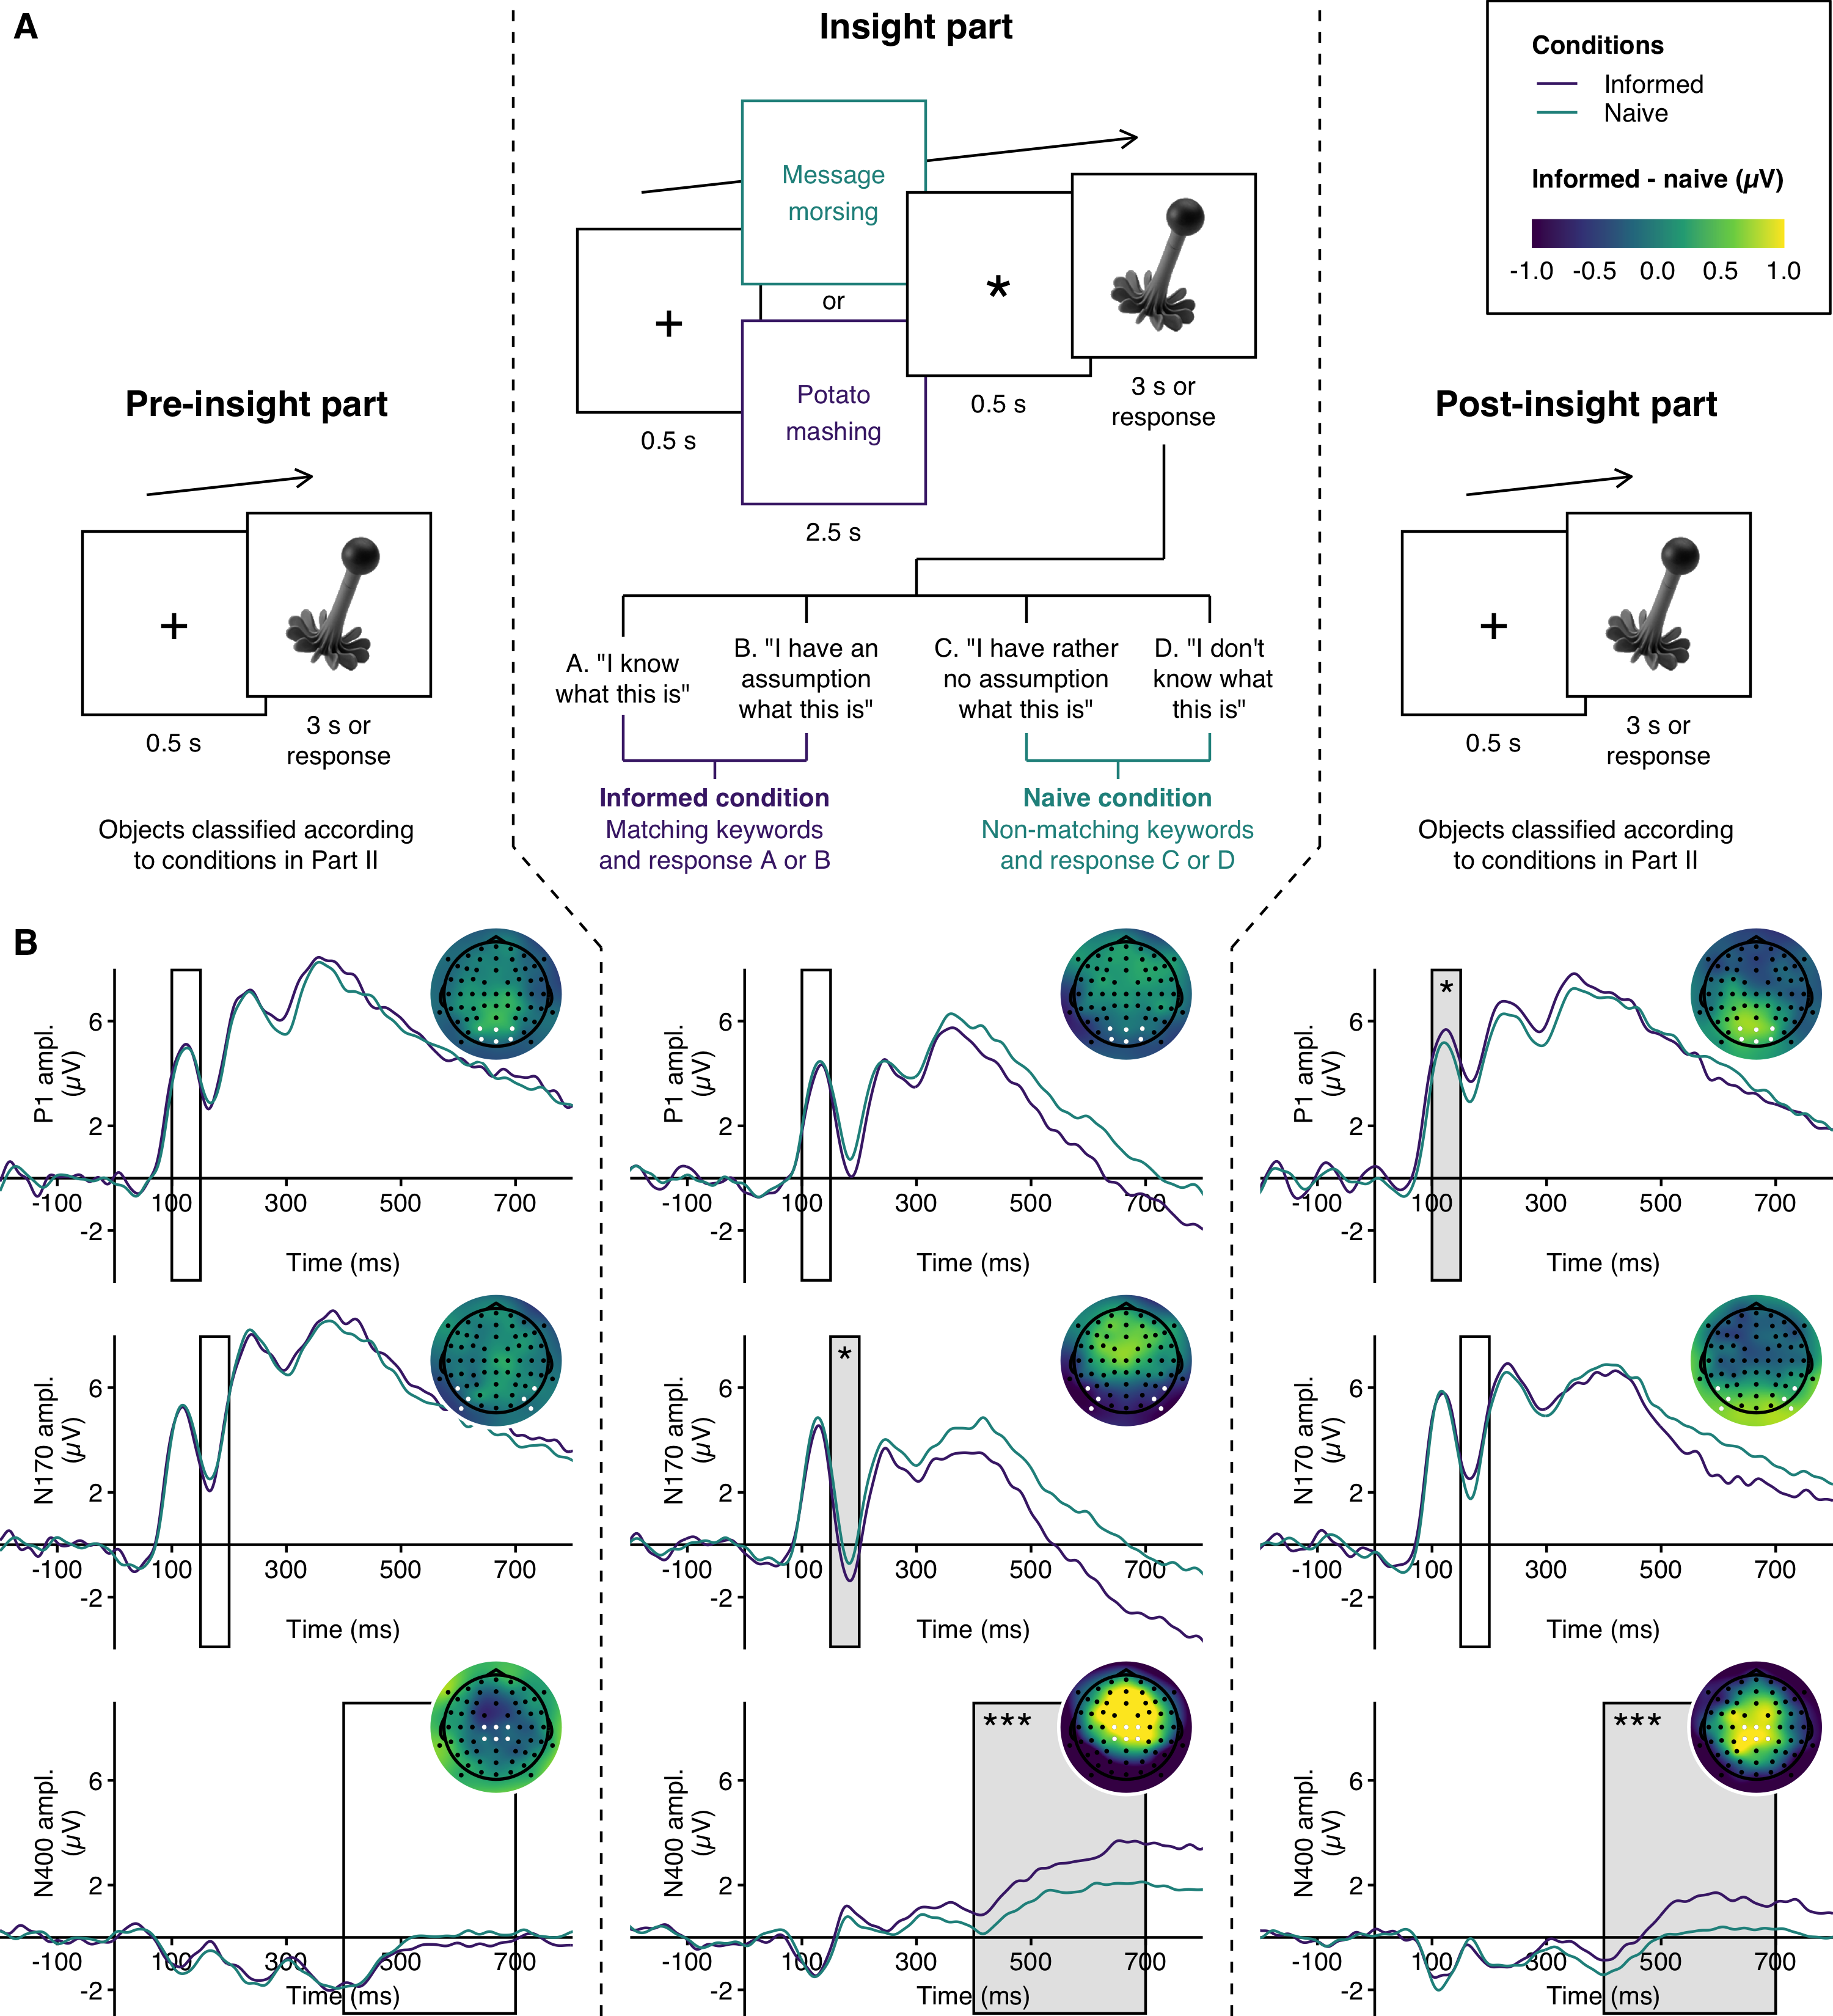
\includegraphics[width=1\linewidth]{master_thesis_files/figure-latex/exp1-plot-1} 

}

\caption{Procedure and Results of Experiment 1\smallskip}\label{fig:exp1-plot}
\end{figure}



In the \emph{insight} part, the 120 unfamiliar objects were presented for a second time, now preceded either by matching keywords (leading to semantically informed perception) or by non-matching keywords (leading to naive perception). Each trial consisted of a fixation cross presented for 0.5 s, followed by the presentation of the keywords for 2.5 s. Then, an asterisk was presented in the middle of the screen for another 0.5 s, followed by the presentation of the object until a response was made or until a time out after 3 s. The objects were presented in blocks of 30 trials so that within each block (a) there were 15 objects from each of the two experimental conditions and (b) objects were heterogeneous in terms of their shape, visual complexity, and functional category (e.g., medical devices, musical instruments).

Finally, in the \emph{post-insight} part, the unfamiliar objects were presented for a third time with an identical trial structure as in the pre-insight part, that is, without any keywords. Note that the insight and post-insight parts were presented in an interleaved fashion so that after the presentation of one block of 30 objects in the insight part (with keywords), participants took a self-timed break and continued with the same block of 30 objects in the post-insight part (without keywords) before moving on to the next block consisting of 30 different objects. They continued like this until all four blocks were completed in both parts. In total, the experiment consisted of 480 trials (120 familiar objects in the pre-insight part and 120 unfamiliar objects in the pre-insight, insight, and post-insight parts). It took participants approximately 35 minutes to complete.

\hypertarget{eeg-recording-and-preprocessing}{%
\subsubsection{EEG Recording and Preprocessing}\label{eeg-recording-and-preprocessing}}

The continuous EEG was recorded from 62 Ag/AgCl scalp electrodes placed according to the extended 10--20 system (American Electroencephalographic Society, 1991) and referenced online to an external electrode placed on the left mastoid (M1). Two additional external electrodes were placed on the right mastoid (M2) and below the left eye (IO1), respectively. During the recording, electrode impedance was kept below 5 kΩ. An online band-pass filter with a high-pass time-constant of 10 s (0.016 Hz) and a low-pass cutoff frequency of 1000 Hz was applied before digitizing the signal at a sampling rate of 500 Hz.

Offline, the data were preprocessed using the MNE software (Version 0.21.0; Gramfort et al., 2013) in Python (Version 3.8.5; van Rossum \& Drake, 2009). First, all scalp electrodes were re-referenced to the common average. Next, artifacts resulting from blinks and eye movements were removed using independent component analysis (ICA). The first 15 components were extracted by the FastICA algorithm (Hyvärinen, 1999) after temporarily low-pass filtering the data at 1 Hz. Any components showing substantive correlations with either of two virtual EOG channels (VEOG: IO1 - Fp1, HEOG: F9 - F10) were removed automatically using the \emph{find\_bads\_eog} function. After artifact correction, a zero-phase, non-causal FIR filter with a lower pass-band edge at 0.1 Hz (transition bandwidth: 0.1 Hz) and an upper pass-band edge at 30 Hz (transition bandwidth: 7.5 Hz) was applied. Next, the continuous EEG was epoched into segments of 2 s, starting 500 ms before the onset of the visual presentation of each unfamiliar object. The epochs were baseline-corrected by subtracting the average voltage during the 200 ms before stimulus onset. Epochs containing artifacts despite ICA, defined as peak-to-peak amplitudes exceeding 200 µV, were removed from further analysis. This led to the exclusion of an average of 2.4 trials per participant (= 0.7\%; range 0 to 24 trials). Single-trial event-related potentials were computed as the mean amplitude across time windows and regions of interests (ROIs) defined a priori, namely 100--150 ms after object onset at electrodes PO3, PO4, POz, O1, O2, and Oz for the P1 component, 150--200 ms after object onset at electrodes P7, P8, PO7, PO8, PO9, and PO10 for the N170 component, and 400--700 ms after object onset at electrodes C1, C2, Cz, CP1, CP2, and CPz for the N400 component (for the positions of these electrodes on the scalp, see the topographies in Figure \ref{fig:exp1-plot}B).

\hypertarget{statistical-analysis}{%
\subsubsection{Statistical Analysis}\label{statistical-analysis}}

First, because we were interested in the effects of knowledge on perceiving \emph{unfamiliar} objects only, we excluded objects from all further analyses when participants classified them as being known in the pre-insight part (i.e.,~before any keywords were presented). This led to the exclusion of an average of 7.5 objects per participant (= 6.3\% of all unfamiliar objects). Next, to clearly delineate semantically informed and naive perception, the assignment of all other objects to one of these two conditions for statistical analysis was co-determined by our experimental manipulation (matching versus non-matching keywords in the insight part) and the behavioral responses of the participants themselves (see Figure \ref{fig:exp1-plot}A). Objects were assigned to the semantically informed condition only if they were presented with matching keywords \emph{and} if participants indicated knowing what the object was or having an assumption. This was the case for an average of 27.0 objects per participant (= 44.9\% of objects presented with matching keywords). Complementarily, objects were assigned to the naive condition only if they were presented with non-matching keywords \emph{and} if participants indicated not knowing what the object was or having rather no assumption. This was the case for an average of 48.8 objects per participant (= 81.2\% of objects presented with non-matching keywords). Although this assignment was based on the manipulation and responses in the second part---when insight was thought to occur---the same assignment was used to analyze the data from the other two parts. This allowed us to test, on the one hand, if the objects from both conditions differed in important aspects even before any keywords were presented (pre-insight part) and, on the other hand, if the semantic understanding acquired in the insight part had any down-stream effects on the subsequent perception of the objects (post-insight part).

The event-related potentials in response to objects from both conditions and all three parts were analyzed on the single trial level using linear mixed-effects regression models (Baayen et al., 2008; Frömer et al., 2018). For the purpose of the present study, these models have at least three desirable properties compared to traditional approaches such as analyses of variance (ANOVAs) performed on by-participant averages. First, they can leverage all of the information that is present in the data set on the single trial level, some of which would be lost when computing averages. Second, they can account simultaneously for the non-independence of data points coming from the same participant and/or from the same item. In contrast, the neglect of the item as a random variable in by-participant ANOVAs leads to anti-conservative test statistics and strictly does not allow for inferences beyond the stimulus set under study (Bürki et al., 2018; Judd et al., 2012). Finally, mixed-effects models can flexibly deal with unbalanced designs in which the number of trials differs across (combinations of) conditions. Such a situation is inevitable when the assignment of trials to conditions is co-determined by the experimental manipulation and the behavior of participants in response to this manipulation (e.g., Fröber et al., 2017).

Three separate models were computed predicting P1, N170, and N400 mean amplitudes, respectively. All models included three fixed effects: (a) the part of the experiment, coded as a repeated contrast (i.e.,~subtracting the first from the second part and the second from the third part, the intercept being the grand mean across all three parts), (b) the condition of the object, coded as a scaled sum contrast (i.e.,~subtracting the naive condition from the semantically informed condition, the intercept being the grand mean across both conditions), and (c) the two-way interaction of part and condition. For details on these and other contrast coding schemes in linear (mixed-effects) models, please refer to Schad et al. (2020). To determine the random effects structure, we always started with a maximal model containing by-participant and by-item random intercepts and random slopes for all fixed effects (Barr et al., 2013). We then performed a model selection algorithm as proposed by Matuschek et al. (2017) in order to increase statistical power and avoid overparameterization: Iteratively, each random effect was removed and the resulting, more parsimonious model was compared to the previous, more complex model by means of a likelihood ratio test. Only if the parsimonious model explained the data equally well as the complex model (determined by \emph{p} \textgreater{} .20; Matuschek et al., 2017) did we leave the random effect out, otherwise it was kept in the final model (see Appendix B for the formulas after model selection). All models were computed in R (Version 4.0.2; R Core Team, 2020) using the lme4 package (Version 1.1.23; Bates et al., 2015). The optimizer function \emph{bobyqa} with 20,000 iterations was used for maximum likelihood estimation. The model selection algorithm via likelihood ratio tests was performed using the buildmer package (Version 1.7.1; Voeten, 2020).

Finally, to answer our research question of whether or not semantically informed perception had an influence on the ERP components within each part, planned follow-up comparisons were calculated, contrasting the semantically informed against the naive condition within the pre-insight, \mbox{insight}, and post-insight parts. This was achieved using the emmeans package (Version 1.5.0; Lenth, 2020). All \emph{p}-values were computed by approximating the relevant denominator degrees of freedom using Satterthwaite's method as implemented in the lmerTest package (Version 3.1.2; Kuznetsova et al., 2017).

The materials, single trial behavioral and ERP data, and all code for data analysis can be accessed via the Open Science Framework (\url{https://osf.io/uksbc/}). We are not able to share the raw EEG data openly because we did not obtain participants' informed consent to do so.

\hypertarget{results}{%
\subsection{Results}\label{results}}

Single-trial ERPs were analyzed in response to unfamiliar objects before (pre-insight part), while (insight part), and after (post-insight part) participants obtained relevant semantic information about their function. In the insight part, half of the objects were preceded by matching keywords, fostering semantically informed perception. The other half were preceded by non-matching keywords, keeping the perception of the object semantically naive. The objects were analyzed according to this manipulation in combination with participants' self-report in the insight part (see Figure \ref{fig:exp1-plot}A), thereby making sure that semantically informed and naive perception did indeed occur. The analysis focused on differences between these two conditions in the P1 component (100--150 ms) as an index of lower-level visual perception, the N170 component (150--200 ms) as index of higher-level visual perception, and the N400 component (400--700 ms) as an index of semantic processing.

\begin{table}[tbp]

\begin{center}
\begin{threeparttable}

\caption{\label{tab:exp1-table}Results of Linear Mixed-Effects Regression Models for Experiment 1\smallskip}

\footnotesize{

\begin{tabular}{lcccccc}
\toprule
 & \multicolumn{2}{c}{\textbf{P1}} & \multicolumn{2}{c}{\textbf{N170}} & \multicolumn{2}{c}{\textbf{N400}} \\
\cmidrule(r){2-3} \cmidrule(r){4-5} \cmidrule(r){6-7}
\textbf{Fixed effects} & \textit{F} (\textit{df}) & \textit{p} & \textit{F} (\textit{df}) & \textit{p} & \textit{F} (\textit{df}) & \textit{p}\\
\midrule
\,\, Part & 10.89 (2, 24.5) & < .001 & 14.18 (2, 24.9) & < .001 & 32.85 (2, 25.6) & < .001\\
\,\, Condition & 0.60 (1, 5343.5) & .438 & 0.30 (1, 24.2) & .586 & 13.00 (1, 24.4) & .001\\
\,\, Pt. × con. & 2.30 (2, 4605.1) & .100 & 4.84 (2, 4878.2) & .008 & 10.91 (2, 5120.9) & < .001\\
\textbf{Informed - naive} & Est. [CI]; \textit{t} (\textit{df}) & \textit{p} & Est. [CI]; \textit{t} (\textit{df}) & \textit{p} & Est. [CI]; \textit{t} (\textit{df}) & \textit{p}\\ \midrule
\,\, Pre-insight part & \makecell[c]{\Gape[6pt][-2pt]{-0.03 [-0.53, 0.47]}\\\Gape[-2pt][6pt]{-0.11 (4996.8)}} & .913 & \makecell[c]{\Gape[6pt][-2pt]{-0.12 [-0.68, 0.44]}\\\Gape[-2pt][6pt]{-0.43 (88.8)}} & .665 & \makecell[c]{\Gape[6pt][-2pt]{-0.20 [-0.65, 0.26]}\\\Gape[-2pt][6pt]{-0.85 (102.7)}} & .400\\
\,\, Insight part & \makecell[c]{\Gape[6pt][-2pt]{-0.18 [-0.68, 0.32]}\\\Gape[-2pt][6pt]{-0.69 (5310.6)}} & .490 & \makecell[c]{\Gape[6pt][-2pt]{-0.64 [-1.20, -0.08]}\\\Gape[-2pt][6pt]{-2.26 (92.4)}} & .026 & \makecell[c]{\Gape[6pt][-2pt]{ 0.93 [0.48, 1.39]}\\\Gape[-2pt][6pt]{ 4.04 (103.7)}} & < .001\\
\,\, Post-insight part & \makecell[c]{\Gape[6pt][-2pt]{ 0.55 [0.05, 1.05]}\\\Gape[-2pt][6pt]{ 2.16 (4717.7)}} & .031 & \makecell[c]{\Gape[6pt][-2pt]{ 0.43 [-0.14, 0.99]}\\\Gape[-2pt][6pt]{ 1.51 (91.8)}} & .136 & \makecell[c]{\Gape[6pt][-2pt]{ 1.00 [0.54, 1.46]}\\\Gape[-2pt][6pt]{ 4.31 (105.0)}} & < .001\\ \midrule
logLik (\textit{df}) & -16555.1 (13) &  & -16289.6 (17) &  & -15350.3 (17) & \\
RMSE & 5.07 &  & 4.79 &  & 4.05 & \\
Conditional $R^2$ & 0.289 &  & 0.379 &  & 0.207 & \\
Marginal $R^2$ & 0.007 &  & 0.053 &  & 0.048 & \\
\bottomrule
\addlinespace
\end{tabular}

}

\begin{tablenotes}[para]
\normalsize{\textit{Note.} Pt. = part, con. = condition, est. = estimate, CI = 95\% confidence interval.}
\end{tablenotes}

\end{threeparttable}
\end{center}

\end{table}

Averaged across conditions, P1, N170, and N400 amplitudes differed as a function of the part of the experiment, all \emph{F}s ≥ 10.89, all \emph{p}s \textless{} .001 (see Table \ref{tab:exp1-table}). In addition, N400 amplitudes differed between the informed and the naive condition averaged across the three parts of the experiment, \emph{F}(1, 24.4) = 13.00, \emph{p} = .001. Crucially, the part × condition interaction was significant in the N170 component, \emph{F}(2, 4878.2) = 4.84, \emph{p} = .008, and in the N400 component, \emph{F}(2, 5120.9) = 10.91, \emph{p} \textless{} .001, while also showing a weak statistical trend in the P1 component, \emph{F}(2, 4605.1) = 2.30, \emph{p} = .100. To answer our main research question, we decomposed these interactions into the differences between the semantically informed condition and the naive condition within the three different parts of the experiment.

\hypertarget{erps-before-insight-was-occurring}{%
\subsubsection{ERPs Before Insight Was Occurring}\label{erps-before-insight-was-occurring}}

In the pre-insight part, when objects were unfamiliar to participants and presented without keywords, no differences emerged between the semantically informed and the naive condition in the P1, N170, or N400 component, all \emph{p}s ≥ .400 (see Table \ref{tab:exp1-table} and Figure \ref{fig:exp1-plot}B). On the one hand, this was to be expected given that the critical presentation of the keywords (leading to semantically informed vs.~naive perception) had not yet taken place. On the other hand, the absence of reliable differences in this part can be taken as evidence---with the usual caveats when interpreting null effects---that any subsequent effect of the semantic information in the other two parts cannot be accounted for by visual differences between the objects in the two conditions. Although the presentation of matching or non-matching keywords for each object was counterbalanced across participants, the fact that different numbers of objects were assigned to the two conditions based on participants' self-report would have made it possible for such visual differences to emerge as a confounding factor. If they did, however, one would expect to detect these differences even before any keywords were presented, which was apparently not the case.

\hypertarget{erps-while-insight-was-occurring}{%
\subsubsection{ERPs While Insight Was Occurring}\label{erps-while-insight-was-occurring}}

In the insight part, half of the unfamiliar objects were presented with matching keywords (for forming the semantically informed condition) and the other half were presented with non-matching keywords (for forming the naive condition). When semantic information informed the perception of the object, the amplitude of the N170 component was significantly enlarged (i.e.,~more negative), \emph{b} = -0.64 µV, \emph{p} = .026, and the amplitude of the N400 component was significantly reduced (i.e.,~less negative), \emph{b} = 0.93 µV, \emph{p} \textless{} .001, compared to when the object was viewed naively without relevant semantic information. As in the pre-insight part, there were no reliable differences in the P1 component, \emph{b} = -0.18 µV, \emph{p} = .490.

\hypertarget{erps-after-insight-had-occurred}{%
\subsubsection{ERPs After Insight Had Occurred}\label{erps-after-insight-had-occurred}}

In the post-insight part, the unfamiliar objects were presented for a third time, again without the keywords (as in the pre-insight part). This allowed us to test if the semantic information had any lasting effects on the processing of the objects. As in the insight part, the N400 component remained significantly reduced during semantically informed as compared to naive perception, \emph{b} = 1.00 µV, \emph{p} \textless{} .001, whereas the effect in the N170 component did not reoccur, \emph{b} = 0.43 µV, \emph{p} = .136. Instead, we now observed an even earlier modulation in the P1 component which was significantly enlarged (i.e.,~more positive) in response to objects for which semantically informed perception had taken place, \emph{b} = 0.55 µV, \emph{p} = .031.

\hypertarget{discussion}{%
\subsection{Discussion}\label{discussion}}

In Experiment 1, we measured the ERPs of participants viewing unfamiliar objects before (pre-insight part), while (insight part) and after (post-insight part) they were able to understand what kind of object they were seeing. To induce this semantically informed perception, half of the objects in the insight part were preceded by matching verbal keywords about the object's typical function or use, whereas the other half were preceded by non-matching keywords, serving as a naive baseline condition.

In the insight part, we found that semantically informed perception was associated with enlarged amplitudes in the N170 component (150--200 ms after object onset) and reduced amplitudes in the N400 component (400--700 ms). When the same objects were presented once more in the post-insight part, the reduction of the N400 component reoccurred and we also observed a modulation of the P1 component (100--150 ms), which was significantly larger for objects for which semantically informed perception had taken place.

Because of the novelty of our experimental paradigm---measuring the ERPs while rather than after participants received semantic information about unfamiliar objects---and because of the novelty of our findings, we ran a replication study with another sample of participants to assess the robustness of these effects.

\hypertarget{experiment-2}{%
\section{Experiment 2}\label{experiment-2}}

\hypertarget{method-1}{%
\subsection{Method}\label{method-1}}

\hypertarget{participants-1}{%
\subsubsection{Participants}\label{participants-1}}

Participants for Experiment 2 were 24 German native speakers (15 female, 9 male) with a mean age of 26 years (range 19 to 29 years) who had not participated in Experiment 1. They had no history of psychological disorders or treatment, were right-handed, and reported normal or corrected-to-normal vision. They gave written informed consent before starting the experiment and received a compensation of €8 per hour for participating.

\hypertarget{materials-procedure-and-analysis}{%
\subsubsection{Materials, Procedure, and Analysis}\label{materials-procedure-and-analysis}}

All materials, procedures, EEG-related methods, and statistical analyses were identical to Experiment 1. An average of 7.0 objects per participant (= 5.8\% of all unfamiliar objects) was classified as being known in the pre-insight part and excluded from all further analyses. Based on participants' responses in the insight part, an average of 26.4 objects was assigned to the semantically informed condition (= 44.0\% of objects presented with matching keywords) and an average of 49.2 objects was assigned to the naive condition (= 82.0\% of objects presented with non-matching keywords). Automatic rejection of EEG epochs containing artifacts led to the exclusion of 11.0 trials per participant (= 3.0\%; range 0 to 85 trials).

\hypertarget{results-1}{%
\subsection{Results}\label{results-1}}

\begin{table}[tbp]

\begin{center}
\begin{threeparttable}

\caption{\label{tab:exp2-table}Results of Linear Mixed-Effects Regression Models for Experiment 2\smallskip}

\footnotesize{

\begin{tabular}{lcccccc}
\toprule
 & \multicolumn{2}{c}{\textbf{P1}} & \multicolumn{2}{c}{\textbf{N170}} & \multicolumn{2}{c}{\textbf{N400}} \\
\cmidrule(r){2-3} \cmidrule(r){4-5} \cmidrule(r){6-7}
\textbf{Fixed effects} & \textit{F} (\textit{df}) & \textit{p} & \textit{F} (\textit{df}) & \textit{p} & \textit{F} (\textit{df}) & \textit{p}\\
\midrule
\,\, Part & 17.45 (2, 5267.1) & < .001 & 16.57 (2, 25.1) & < .001 & 70.12 (2, 25.2) & < .001\\
\,\, Condition & 0.02 (1, 5276.9) & .900 & 0.98 (1, 5228.5) & .322 & 19.95 (1, 5242.5) & < .001\\
\,\, Pt. × con. & 3.60 (2, 5267.1) & .027 & 1.25 (2, 4756.5) & .287 & 7.92 (2, 4714.9) & < .001\\
\textbf{Informed - naive} & Est. [CI]; \textit{t} (\textit{df}) & \textit{p} & Est. [CI]; \textit{t} (\textit{df}) & \textit{p} & Est. [CI]; \textit{t} (\textit{df}) & \textit{p}\\ \midrule
\,\, Pre-insight part & \makecell[c]{\Gape[6pt][-2pt]{-0.16 [-0.71, 0.40]}\\\Gape[-2pt][6pt]{-0.55 (5270.9)}} & .582 & \makecell[c]{\Gape[6pt][-2pt]{-0.03 [-0.53, 0.48]}\\\Gape[-2pt][6pt]{-0.10 (4772.1)}} & .920 & \makecell[c]{\Gape[6pt][-2pt]{0.04 [-0.43, 0.50]}\\\Gape[-2pt][6pt]{0.15 (5177.9)}} & .877\\
\,\, Insight part & \makecell[c]{\Gape[6pt][-2pt]{-0.48 [-1.03, 0.08]}\\\Gape[-2pt][6pt]{-1.67 (5270.7)}} & .094 & \makecell[c]{\Gape[6pt][-2pt]{-0.48 [-0.99, 0.03]}\\\Gape[-2pt][6pt]{-1.85 (5241.8)}} & .064 & \makecell[c]{\Gape[6pt][-2pt]{1.33 [0.87, 1.79]}\\\Gape[-2pt][6pt]{5.68 (4781.9)}} & < .001\\
\,\, Post-insight part & \makecell[c]{\Gape[6pt][-2pt]{ 0.57 [0.01, 1.13]}\\\Gape[-2pt][6pt]{ 1.99 (5270.8)}} & .047 & \makecell[c]{\Gape[6pt][-2pt]{ 0.06 [-0.45, 0.57]}\\\Gape[-2pt][6pt]{ 0.23 (5035.9)}} & .818 & \makecell[c]{\Gape[6pt][-2pt]{0.47 [0.01, 0.93]}\\\Gape[-2pt][6pt]{1.98 (5067.3)}} & .047\\ \midrule
logLik (\textit{df}) & -16707.1 (8) &  & -16174.3 (13) &  & -15648.0 (13) & \\
RMSE & 5.62 &  & 5.03 &  & 4.58 & \\
Conditional $R^2$ & 0.242 &  & 0.399 &  & 0.174 & \\
Marginal $R^2$ & 0.005 &  & 0.037 &  & 0.068 & \\
\bottomrule
\addlinespace
\end{tabular}

}

\begin{tablenotes}[para]
\normalsize{\textit{Note.} Pt. = part, con. = condition, est. = estimate, CI = 95\% confidence interval.}
\end{tablenotes}

\end{threeparttable}
\end{center}

\end{table}

As in Experiment 1, P1, N170, and N400 amplitudes differed between the three different parts of the experiments, all \emph{F}s ≥ 16.57, all \emph{p}s \textless{} .001 (see Table \ref{tab:exp2-table}). Also as in Experiment 1, N400 amplitudes differed between the informed and the naive condition averaged across parts, \emph{F}(1, 5242.5) = 19.95, \emph{p} \textless{} .001. The part × condition interaction was significant in the P1 component, \emph{F}(2, 5267.1) = 3.60, \emph{p} = .027, and in the N400 component, \emph{F}(2, 4714.9) = 7.92, \emph{p} \textless{} .001, but not in the N170 component, \emph{F}(2, 4756.5) = 1.25, \emph{p} = .287.

\begin{figure}

{\centering 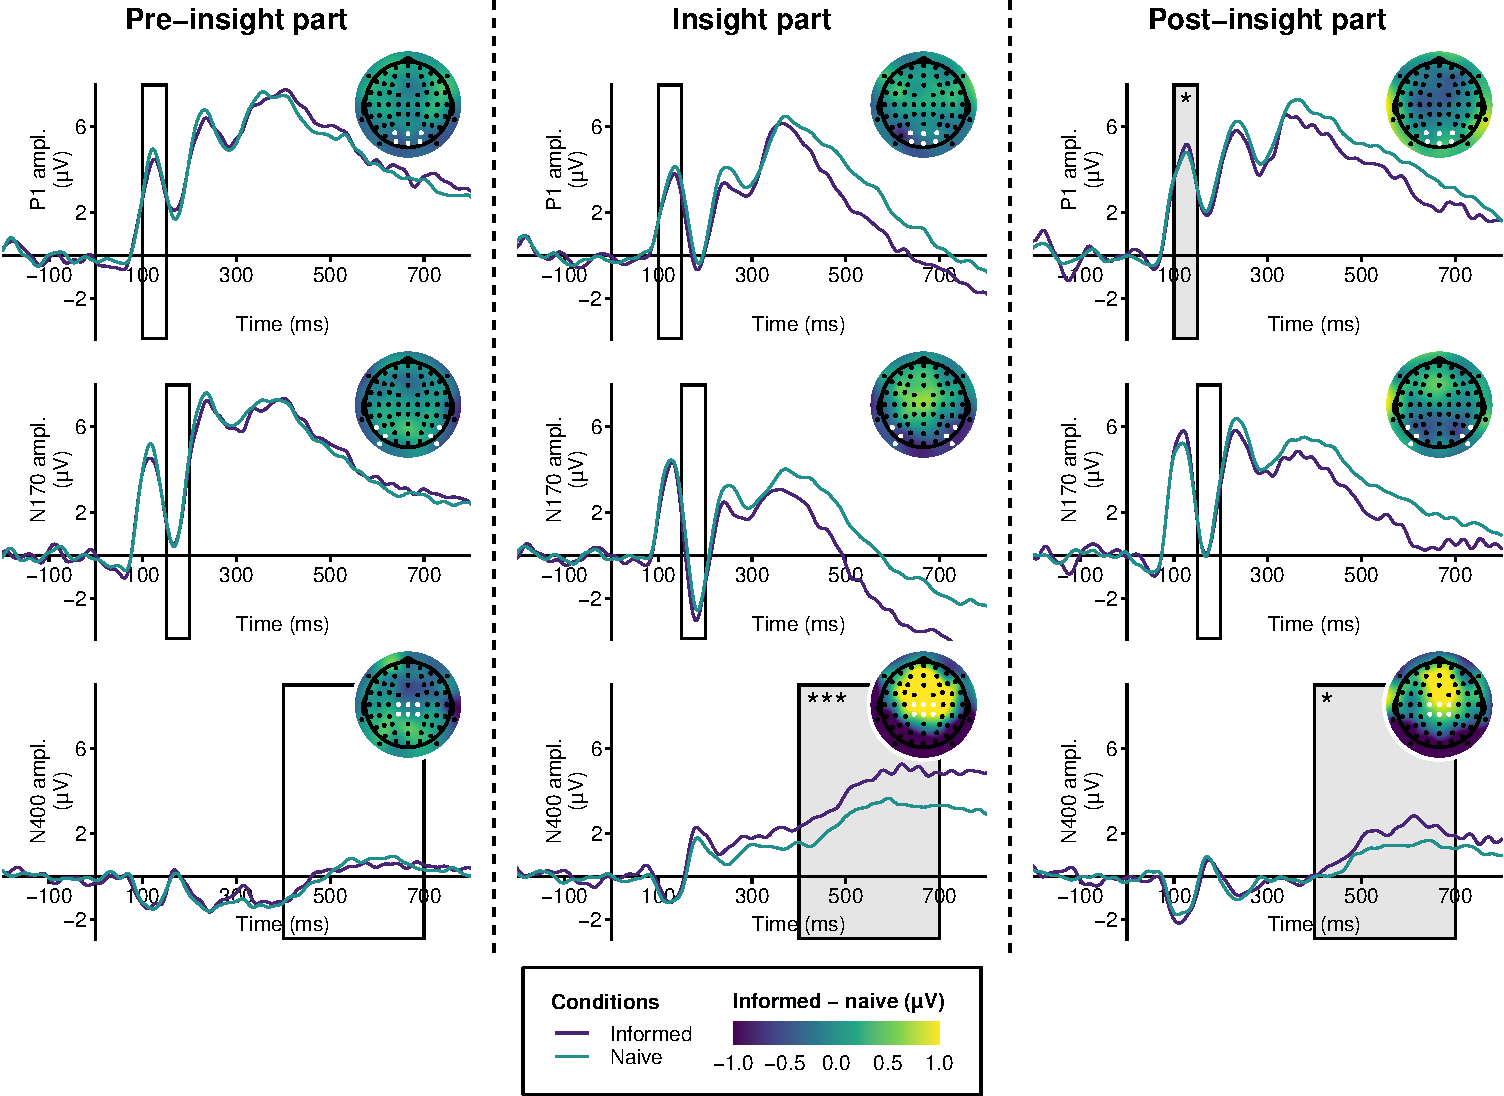
\includegraphics[width=1\linewidth]{master_thesis_files/figure-latex/exp2-plot-1} 

}

\caption{Results of Experiment 2\smallskip}\label{fig:exp2-plot}
\end{figure}



\hypertarget{erps-before-insight-was-occurring-1}{%
\subsubsection{ERPs Before Insight Was Occurring}\label{erps-before-insight-was-occurring-1}}

As in Experiment 1, no differences between objects in the semantically informed and the naive condition emerged in the P1, N170, or N400 component, all \emph{p}s ≥ .582 (see Table \ref{tab:exp2-table} and Figure \ref{fig:exp2-plot}).

\hypertarget{erps-while-insight-was-occurring-1}{%
\subsubsection{ERPs While Insight Was Occurring}\label{erps-while-insight-was-occurring-1}}

As in Experiment 1, semantically informed as compared to naive perception (induced by matching vs.~non-matching keywords) was associated with an enhancement of the N170 component, although this effect marginally failed to reach statistical significance, \emph{b} = -0.48 µV, \emph{p} = .064. The reduction of the N400 component during semantically informed perception remained significant, \emph{b} = 1.33 µV, \emph{p} \textless{} .001.

\hypertarget{erps-after-insight-had-occurred-1}{%
\subsubsection{ERPs After Insight Had Occurred}\label{erps-after-insight-had-occurred-1}}

As in Experiment 1, the presentation of the same unfamiliar objects for a third time (without keywords, as in the pre-insight part) again led to significantly reduced amplitudes in the N400 component in response to objects for which semantically informed perception had occurred, \emph{b} = 0.47 µV, \emph{p} = .047. Also, P1 amplitudes in response these objects were significantly enlarged, \emph{b} = 0.57 µV, \emph{p} = .047.

\hypertarget{joint-analysis-of-experiments-1-and-2}{%
\subsubsection{Joint Analysis of Experiments 1 and 2}\label{joint-analysis-of-experiments-1-and-2}}

In an attempt to maximize statistical power, we combined the ERP data sets from Experiments 1 and 2. This allowed us to determine (a) if the above effects---including the marginally significant ones---were reliable when tested in a larger sample, and (b) if there were significant differences in the ERP amplitudes between Experiments 1 and 2. Methods for statistical analysis were kept unchanged apart from the addition of a new factor denoting the experiment, coded as a scaled sum contrast (i.e.,~subtracting Experiment 1 from Experiment 2, the intercept being the grand mean across both experiments; Schad et al., 2020). This factor and its interactions with part, condition, and part × condition were included in the linear mixed-effects regression models as fixed effects and as potential by-item random slopes. They were not included as by-participant random slopes because different participants took part in Experiments 1 and 2. Note that, as above, random effects were eventually included only if their omission led to a significant decline in model fit (Matuschek et al., 2017; Voeten, 2020). The resulting formulas for the models can be found in Appendix B.

\begin{table}[tbp]

\begin{center}
\begin{threeparttable}

\caption{\label{tab:joint-table}Results of Linear Mixed-Effects Regression Models for Experiments 1 and 2 Combined\smallskip}

\footnotesize{

\begin{tabular}{lcccccc}
\toprule
 & \multicolumn{2}{c}{\textbf{P1}} & \multicolumn{2}{c}{\textbf{N170}} & \multicolumn{2}{c}{\textbf{N400}} \\
\cmidrule(r){2-3} \cmidrule(r){4-5} \cmidrule(r){6-7}
\textbf{Fixed effects} & \textit{F} (\textit{df}) & \textit{p} & \textit{F} (\textit{df}) & \textit{p} & \textit{F} (\textit{df}) & \textit{p}\\
\midrule
\,\, Part & 12.34 (2, 49.1) & < .001 & 30.08 (2, 50.3) & < .001 & 94.61 (2, 50.6) & < .001\\
\,\, Condition & 0.15 (1, 10573.1) & .699 & 1.16 (1, 45.2) & .287 & 41.38 (1, 10593.6) & < .001\\
\,\, Experiment & 0.33 (1, 48.2) & .567 & 2.50 (1, 48.0) & .121 & 4.96 (1, 48.4) & .031\\
\,\, Pt. × con. & 3.90 (2, 9004.9) & .020 & 5.26 (2, 9904.1) & .005 & 15.34 (2, 10091.0) & < .001\\
\,\, Pt. × exp. & 0.04 (2, 49.1) & .966 & 0.58 (2, 50.3) & .565 & 2.55 (2, 50.6) & .088\\
\,\, Ins. × exp. & 0.43 (1, 10573.1) & .514 & 0.06 (1, 45.2) & .805 & 0.07 (1, 10593.6) & .785\\
\,\, Pt. × con. × exp. & 0.03 (2, 9004.9) & .968 & 0.58 (2, 9904.1) & .559 & 2.54 (2, 10091.0) & .079\\
\textbf{Informed - naive} & Est. [CI]; \textit{t} (\textit{df}) & \textit{p} & Est. [CI]; \textit{t} (\textit{df}) & \textit{p} & Est. [CI]; \textit{t} (\textit{df}) & \textit{p}\\ \midrule
\,\, Pre-insight part & \makecell[c]{\Gape[6pt][-2pt]{-0.10 [-0.47, 0.28]}\\\Gape[-2pt][6pt]{-0.50 (9534.6)}} & .616 & \makecell[c]{\Gape[6pt][-2pt]{-0.10 [-0.48, 0.29]}\\\Gape[-2pt][6pt]{-0.51 (208.1)}} & .611 & \makecell[c]{\Gape[6pt][-2pt]{-0.09 [-0.39, 0.22]}\\\Gape[-2pt][6pt]{-0.56 (10459.4)}} & .577\\
\,\, Insight part & \makecell[c]{\Gape[6pt][-2pt]{-0.24 [-0.62, 0.13]}\\\Gape[-2pt][6pt]{-1.28 (10420.2)}} & .202 & \makecell[c]{\Gape[6pt][-2pt]{-0.57 [-0.96, -0.18]}\\\Gape[-2pt][6pt]{-2.90 (214.4)}} & .004 & \makecell[c]{\Gape[6pt][-2pt]{ 1.10 [0.80, 1.41]}\\\Gape[-2pt][6pt]{ 7.09 (10436.6)}} & < .001\\
\,\, Post-insight part & \makecell[c]{\Gape[6pt][-2pt]{ 0.47 [0.09, 0.84]}\\\Gape[-2pt][6pt]{ 2.45 (9881.6)}} & .014 & \makecell[c]{\Gape[6pt][-2pt]{ 0.24 [-0.15, 0.63]}\\\Gape[-2pt][6pt]{ 1.22 (211.4)}} & .225 & \makecell[c]{\Gape[6pt][-2pt]{ 0.73 [0.42, 1.04]}\\\Gape[-2pt][6pt]{ 4.67 (10339.5)}} & < .001\\ \midrule
logLik (\textit{df}) & -33272.6 (19) &  & -32474.6 (23) &  & -31045.5 (19) & \\
RMSE & 5.32 &  & 4.91 &  & 4.32 & \\
Conditional $R^2$ & 0.271 &  & 0.400 &  & 0.198 & \\
Marginal $R^2$ & 0.008 &  & 0.06 &  & 0.07 & \\
\bottomrule
\addlinespace
\end{tabular}

}

\begin{tablenotes}[para]
\normalsize{\textit{Note.} Pt. = part, con. = condition, exp. = experiment, est. = estimate, CI = 95\% confidence interval.}
\end{tablenotes}

\end{threeparttable}
\end{center}

\end{table}

As shown in Table \ref{tab:joint-table}, the main effect of part was significant in the P1, N170, and N400 component, all \emph{F}s ≥ 12.34, all \emph{p}s \textless{} .001, as was the main effect of condition in the N400, \emph{F}(1, 10593.6) = 41.38, \emph{p} \textless{} .001. Furthermore, the part × condition interaction was now observed reliably in all three components, all \emph{F}s ≥ 3.90, all \emph{p}s ≤ .020. There was a main effect of experiment in the N400, \emph{F}(1, 48.4) = 4.96, \emph{p} = .031, with more negative amplitudes in Experiment 1 as compared to Experiment 2, \emph{b} = -1.06. However, the absence of any significant interactions of experiment with part or condition indicated that the effects of our experimental manipulations did not differ between Experiments 1 and 2.

Based on the part × condition interaction, we again computed follow-up comparisons between the semantically informed and the naive condition within each part, now collapsed across the data from both experiments (see Table \ref{tab:joint-table} and Figure \ref{fig:joint-plot}). This confirmed the absence of any reliable differences between the two conditions in the pre-insight part, all \emph{p}s ≥ .577, the significant enhancement of the N170 component in the insight part, while the semantic information was obtained, \emph{b} = -0.57 µV, \emph{p} = .004, the significant reduction of the N400 component in the insight part, while the semantic information was obtained, \emph{b} = 1.10 µV, \emph{p} \textless{} .001, and in the post-insight part, after the information had been obtained, \emph{b} = 0.73 µV, \emph{p} \textless{} .001, as well as the significant enhancement of the P1 component in the post-insight part, after the information had been obtained, \emph{b} = 0.47 µV, \emph{p} = .014.



\begin{figure}

{\centering 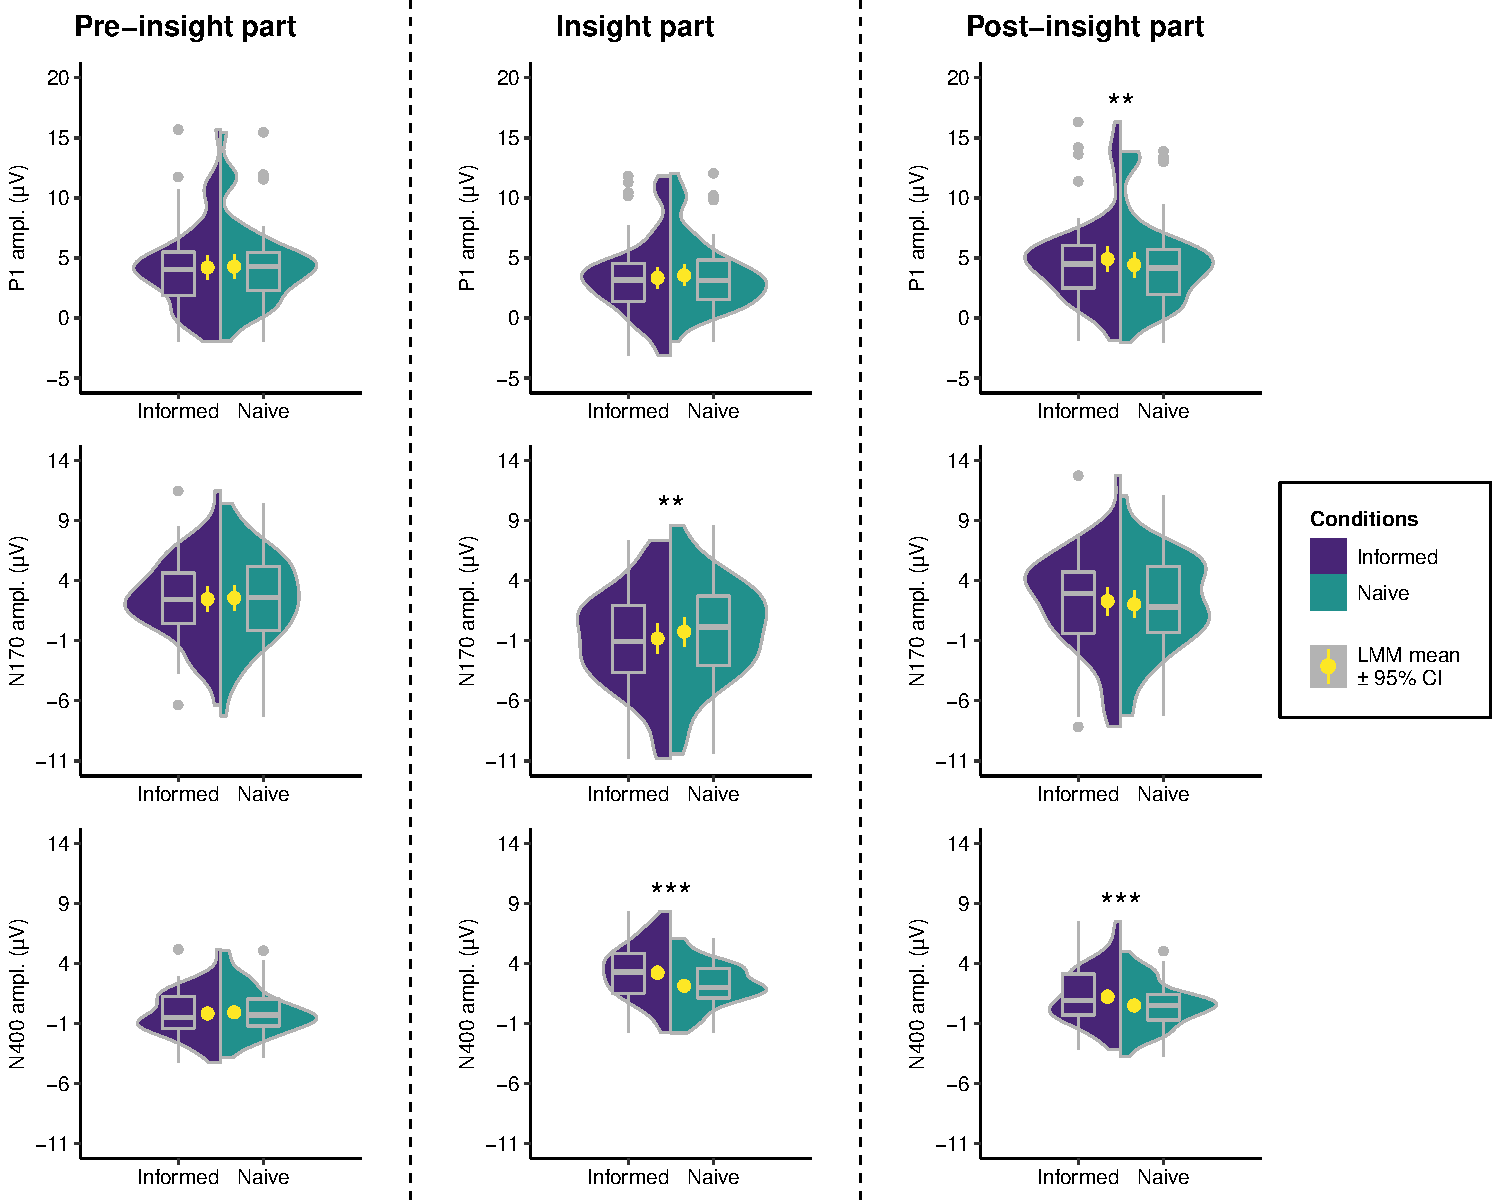
\includegraphics[width=1\linewidth]{master_thesis_files/figure-latex/joint-plot-1} 

}

\caption{Measured and Modeled ERP Amplitudes for Experiments 1 and 2 Combined\smallskip}\label{fig:joint-plot}
\end{figure}

\hypertarget{control-analysis}{%
\subsubsection{Control Analysis}\label{control-analysis}}

One may raise concerns whether the modulation of the N170 component in the insight part genuinely reflects the semantically informed perception of the objects in the respective condition, or---as an alternative explanation---whether it may be driven by the objects in the other, semantically naive condition. Remember that these objects were preceded by non-matching keywords which were picked so that they could not be related to the visual features of the object and their configuration. Thus, the modulation of the ERP components in the insight part could be a mismatch response to those objects---reflecting, for example, the fact that the visual features of the object shown in Figure \ref{fig:exp1-plot}A cannot be reconciled with the function of signalling messages. To preclude this alternative explanation, we repeated our analysis using a different baseline against which the objects in the semantically informed condition were contrasted. Instead of the naive condition (where objects were presented with non-matching keywords), we now used those objects which were presented with matching keywords (as in the informed condition), but which were excluded from the main analysis because participants indicated behaviorally that they did not understand the object they were seeing. Across both experiments, this was the case for 49.6\% of objects presented with matching keywords, as compared to 44.4\% of objects which did indeed lead to semantically informed perception.\footnote{Note that these percentages do not add up to 100\% because some objects were excluded from all analyses if participants indicated knowing these objects in the pre-insight part, before any keywords had been presented (see Method).} Just as above, this control analysis revealed a robust N170 effect in the insight part, \emph{b} = -1.00 µV, \emph{p} \textless{} .001. Thus, this enhanced negativity seems to be a genuine marker of semantically informed perception, no matter if compared to objects presented with non-matching keywords or compared to objects presented with matching keywords on which participants failed to capitalize. Note that the reduction of the N400 component in the insight part also remained robust in this control analysis, \emph{b} = 1.25 µV, \emph{p} \textless{} .001.

\hypertarget{discussion-1}{%
\subsection{Discussion}\label{discussion-1}}

Experiment 2, which was an exact replication of Experiment 1, confirmed the effects of obtaining semantic information about previously unfamiliar objects on ERPs associated with lower-level visual perception (P1), higher-level visual perception (N170), and semantic processing (N400). Objects for which participants experienced semantically informed perception via matching keywords elicited enlarged N170 amplitudes and reduced N400 amplitudes. Note, however, that the effect in the N170 component marginally failed to reach the conventional level for statistical significance in this replication experiment. When the objects were presented once more without any semantic information, they again elicited reduced N400 amplitudes as well as enlarged P1 amplitudes.

\hypertarget{general-discussion}{%
\section{General Discussion}\label{general-discussion}}

Here we investigated if obtaining a semantic understanding of previously unfamiliar objects has an influence on how we perceive them. To this end, we measured ERPs while participants viewed unfamiliar objects before, while, and after receiving semantic information about them. For half of the objects, this information was matching the object, thus leading to semantically informed perception, whereas for the other half of the objects, the information was non-matching, thus keeping the perception of the object semantically naive. We found semantically informed perception to be accompanied by enlarged (i.e., more negative) N170 amplitudes and reduced (i.e., less negative) N400 amplitudes. When the same objects were presented again without the semantic information, the N400 component remained significantly reduced and we also observed a modulation of the P1 component, which was enlarged (i.e., more positive) in response to objects that had previously triggered semantically informed perception. We will discuss each of these effects in turn, starting with the latest (i.e., post-perceptual) effect and moving backward in time to the earlier (i.e., more perceptual) effects.

The reduction of the N400 component (400--700 ms after object onset) during semantically informed perception was the numerically largest and most robust effect. Perhaps least controversially, this effect indicates that acquiring an understanding of the objects (in the insight part) lessened participants' demand for effortful semantic processing in comparison to the naive condition (Kutas \& Federmeier, 2011). This replicates previous work showing that N400 amplitudes are larger in response to pictures when they are either difficult to understand in and of themselves (e.g., Abdel Rahman \& Sommer, 2008; Supp et al., 2005) or difficult to integrate into the preceding context (e.g., Barrett \& Rugg, 1990; Ganis et al., 1996; Hirschfeld et al., 2011). The time course of this effect and the computational role of the N400 (Lau et al., 2008; Rabovsky et al., 2018) suggest that it has a post-perceptual locus.

In contrast to the N400, the N170 component (150--200 ms after object onset) was modulated while but not after the objects were presented together with the relevant semantic information. As such, it can be seen as an online marker of semantic insight, that is, participants suddenly understanding the visual objects in the light of the additional information provided by the verbal keywords. The N170 is typically associated with the holistic perception of faces (Eimer et al., 2011; Sagiv \& Bentin, 2001) and other stimuli of visual expertise (Rossion et al., 2002; Tanaka \& Curran, 2001). It being enlarged during semantically informed perception may therefore reflect that the additional semantic information made participants experience the configuration of the visual features of the objects in a new and meaningful way. This interpretation is supported by previous findings with a similar experimental paradigm in the domain of face perception (Bentin \& Golland, 2002): In this study, participants showed a face-like (i.e., enlarged) N170 response to a scrambled version of a schematic face after (but not before) they were primed with the intact version of the same face. This effect was absent when a visual control stimulus (a non-face object) was shown instead of the intact face. In the domain of non-face stimuli, enlarged N170 amplitudes have also been observed when participants were asked to discriminate between composite line drawings of meaningful objects as compared to composite line drawings of non-objects (Beaucousin et al., 2011). Of note, this effect was present only when participants were asked to decide based on the global shape of the object and it was reversed in polarity when they were asked to decide based on the constituent parts of the object. Together with the present study, these findings suggest an online impact of meaningfulness on the higher-level (i.e., holistic) perception of visual objects, integrating across their visual features.

The P1 component (100--150 ms after object onset), unlike the N400 and N170 components, was modulated by semantic information only one trial after the information had been obtained. This is consistent with previous studies showing modulations of the P1 component when participants learned meaningful information about previously unfamiliar objects (Abdel Rahman \& Sommer, 2008; Maier \& Abdel Rahman, 2019, 2018; Weller et al., 2019) or about familiar objects that were rendered difficult to recognize (Samaha et al., 2018). What the present study adds to these findings is that the P1 effect does not take an extensive learning phase to develop (with multiple presentations of the objects together with the respective information). Instead, it can be observed as soon as one trial after semantic insight has happened. Because the P1 is typically associated with lower-level sensory processing (e.g., Johannes et al., 1995; Luck, 2014; Pratt, 2011), we take its susceptibility to semantic information as an indicator that knowledge about the function of an object can change how we perceive it visually.

Both the N170 and the P1 components therefore seem to be sensitive to the semantic meaningfulness of visual objects. However, the finding that these two components were modulated in different parts of our experimental design suggests that they reflect different aspects of top-down processing with different time courses and neuroanatomical implementations. It has been pointed out that the time course of the N170 component is consistent with a top-down influence of (non-visual) areas in the prefrontal and parietal cortices on visual areas, whereas modulations of the P1 component seem reflect recurrent processing \emph{within} the visual system (Wyatte et al., 2014). Here we could show that the former pathway seems to be able to convey semantic information instantaneously (i.e., within the same trial), whereas the latter seems to take at least one---but apparently also not more than one---additional presentation of the visual object to emerge.

While the limited spatial resolution of the EEG precludes a precise localization of these effects within the ventral stream of object recognition, there is converging evidence coming from fMRI showing that semantic information can feed back into the earliest of visual areas. Hsieh et al. (2010) showed participants indiscernible two-tone (``Mooney'') versions of images before and after showing them the original versions. They found that the brain responses to the original image were correlated more strongly with the second presentation of the Mooney image (after insight had taken place) than with the first presentation of the Mooney image (before insight had taken place). This increase in representational similarity was not just observed in higher-level object-sensitive areas in the lateral occipital cortex (LOC), but also in early retinotopic cortex (areas V1, V2, and V3). Both of these cortical regions are consistent with the neural generators of the N170 and P1 components of the ERP which we have found to be sensitive to the semantically informed perception of previously unfamiliar objects.

On a theoretical level, the top-down modulation of these visual ERPs by semantic information challenges a modular view of visual perception (Firestone \& Scholl, 2016; Fodor, 1983; Pylyshyn, 1999; but see Clarke, 2020). However, proponents of such a modular view have pointed out important shortcomings of previous studies that claimed to demonstrate top-down effects of cognition on perception (Firestone \& Scholl, 2016; Machery, 2015). We took care to address as many of these shortcomings as possible: First, we showed that no effect had been present before any semantic information was being presented (in the pre-insight part). Second, we used an objective and time-resolved measure (ERPs) to disentangle effects with a perceptual locus from those with a post-perceptual locus. Third, we reduced response and demand biases by keeping the manipulation (i.e., matching or non-matching keywords) obscure to the participants and by including well-known objects as filler stimuli. Fourth, we precluded low-level visual differences between conditions by counterbalancing the assignment of objects to conditions across participants. Fifth, we reduced priming and attentional effects by presenting all objects in a randomized order and at the same location. Sixth, we reduced memory effects by using only unfamiliar objects and by measuring online ERPs rather than delayed behavioral responses. We hope that these procedures have effectively ruled out some of the most important alternative explanations for the top-down effects that we have observed, thus making a more compelling case against the cognitive impenetrability of perception.

An interactive view of object vision with an abundance of top-down feedback also challenges the predominantly feed-forward models in computer vision (e.g., Marr, 1982; Serre et al., 2007). In fact, the lack of a semantic knowledge base that dynamically interacts with the processing of lower-level visual features may be one key reason why even state-of-the-art deep-learning algorithms need orders of magnitude more training examples to achieve human-level performance in object recognition. For these network models, single-trial learning of previously unfamiliar objects, as was observed on the behavioral and on the neurophysiological level in the present study, seems to be out of reach until they overcome this ``barrier of meaning'' (Mitchell, 2020). Drawing inspiration from cognitive psychology and human neuroscientific data may help to make these models more biologically plausible and, at the same time, more data efficient.

A theoretical framework that would explicitly predict or explain the observed P1 and N170 effects in our study is lacking at present. The effects are consistent, however, with the reverse hierarchy theory (Ahissar \& Hochstein, 2004; Hochstein \& Ahissar, 2002) which posits that objects first enter our visual consciousness at an abstract, conceptual level. Once this initial ``vision at a glance'' has taken place, feedback connections to earlier layers of the visual system are being accessed to extract the relevant lower-level features (``vision with scrutiny''). This reverse trajectory down the visual hierarchy may explain (a) the semantically induced changes to the fMRI signal in LOC and retinotopic cortex (Hsieh et al., 2010) as well as (b) the modulations of early visual ERP components observed in the present study and others (Abdel Rahman \& Sommer, 2008; Maier et al., 2014; Maier \& Abdel Rahman, 2019; Samaha et al., 2018; Weller et al., 2019). Besides this specific theory, an important role of top-down mechanisms for vision or, more specifically, object recognition is also posited by the family of predictive coding and Bayesian inference theories (e.g., Clark, 2013; Lupyan, 2015; Panichello et al., 2013; Yuille \& Kersten, 2006). Despite the theoretical advances, the mechanistic details of these top-down effects at the algorithmic and implementational level (Marr, 1982) remain to be clarified.

The lack of mechanistic insight into the top-down effects that we have observed is one limitation of the present study. Another one is our reliance on rare and highly specialized objects (see Appendix A). This was necessary to induce the experience of semantic insight in a population of undergraduate students but the results may not necessarily generalize to the way in which we learn about everyday objects.\footnote{Note, however, the converging evidence coming from the complementary approach of rendering images of everyday objects difficult to recognize (Samaha et al., 2018).} One way of addressing this issue would be to adapt the present paradigm to younger participants, using everyday objects which they have not yet learned about. Finally, the number participants (\emph{n} = 24 per experiment) and trials (\emph{k} \(\approx\) 30 per part in the insight condition and \emph{k} \(\approx\) 50 per part in the naive condition) can be considered small by today's standards (Baker et al., 2020). Our analysis may therefore not have been particularly sensitive, especially given that linear mixed-effects regression models tend to have limited statistical power under a wide range of circumstances (see, e.g., the simulations by Matuschek et al., 2017). This lack of power may also explain why one of the effects that had been observed in the first experiment (i.e., the enlargement of the N170 component, \emph{p} = .026) failed to reach statistical significance in the replication experiment (\emph{p} = .064). To discern if this was due to a lack of statistical power or due to the actual absence of an effect, it would take yet another (more highly powered) replication study and/or a different data-analytic approach where it is possible to estimate the evidence both for the alternative hypothesis and for the null hypothesis (e.g., Bayesian linear mixed models). It should be noted, however, that the joint analysis of both data sets yielded a very robust N170 effect (\emph{p} = .004). This makes it less likely that the effect observed in Experiment 1 was due to a false positive and instead suggests that statistical power in Experiment 2 was insufficient to render the effect significant. Also note that the effect in the P1 component was statistically significant in both experiments individually, making an even stronger case for the susceptibility of early cortical processing to newly acquired knowledge about objects.

Taken together, this study provides preliminary evidence that whenever we receive meaningful semantic information about a previously unfamiliar object, this information has an immediate influence on the processing of the object. This influence is immediate in at least two different ways: First, it does not require extensive training and can instead be observed within the same trial in which the information has been presented (and/or one trial later). Second, the time course of this influence suggests that it manifests itself not only at later, post-perceptual stages---typically associated with semantic processing---but also at earlier stages---typically associated with visual perception itself and happening within less than a fifth of a second after the object is presented to us.

\newpage

\hypertarget{references}{%
\section{References}\label{references}}

\setlength{\parindent}{-0.5in}

\raggedright
\setlength{\cslhangindent}{0.5in}

\hypertarget{refs}{}
\begin{CSLReferences}{1}{0}
\leavevmode\hypertarget{ref-abdelrahman2011}{}%
Abdel Rahman, R. (2011). Facing good and evil: Early brain signatures of affective biographical knowledge in face recognition. \emph{Emotion}, \emph{11}(6), 1397--1405. \url{https://doi.org/10.1037/a0024717}

\leavevmode\hypertarget{ref-abdelrahman2008}{}%
Abdel Rahman, R., \& Sommer, W. (2008). Seeing what we know and understand: How knowledge shapes perception. \emph{Psychonomic Bulletin \& Review}, \emph{15}(6), 1055--1063. \url{https://doi.org/10.3758/PBR.15.6.1055}

\leavevmode\hypertarget{ref-ahissar2004}{}%
Ahissar, M., \& Hochstein, S. (2004). The reverse hierarchy theory of visual perceptual learning. \emph{Trends in Cognitive Sciences}, \emph{8}(10), 457--464. \url{https://doi.org/10.1016/j.tics.2004.08.011}

\leavevmode\hypertarget{ref-americanelectroencephalographicsociety1991}{}%
American Electroencephalographic Society. (1991). {American Electroencephalographic Society} guidelines for standard electrode position nomenclature. \emph{Journal of Clinical Neurophysiology}, \emph{8}(2), 200--202.

\leavevmode\hypertarget{ref-baayen2008}{}%
Baayen, R. H., Davidson, D. J., \& Bates, D. M. (2008). Mixed-effects modeling with crossed random effects for subjects and items. \emph{Journal of Memory and Language}, \emph{59}(4), 390--412. \url{https://doi.org/10.1016/j.jml.2007.12.005}

\leavevmode\hypertarget{ref-baker2020}{}%
Baker, D. H., Vilidaite, G., Lygo, F. A., Smith, A. K., Flack, T. R., Gouws, A. D., \& Andrews, T. J. (2020). Power contours: Optimising sample size and precision in experimental psychology and human neuroscience. \emph{Psychological Methods}. \url{https://doi.org/10.1037/met0000337}

\leavevmode\hypertarget{ref-balcetis2010}{}%
Balcetis, E., \& Dunning, D. (2010). Wishful seeing: More desired objects are seen as closer. \emph{Psychological Science}, \emph{21}(1), 147--152. \url{https://doi.org/10.1177/0956797609356283}

\leavevmode\hypertarget{ref-barr2013}{}%
Barr, D. J., Levy, R., Scheepers, C., \& Tily, H. J. (2013). Random effects structure for confirmatory hypothesis testing: Keep it maximal. \emph{Journal of Memory and Language}, \emph{68}(3), 255--278. \url{https://doi.org/10.1016/j.jml.2012.11.001}

\leavevmode\hypertarget{ref-barrett1990}{}%
Barrett, S. E., \& Rugg, M. D. (1990). Event-related potentials and the semantic matching of pictures. \emph{Brain and Cognition}, \emph{14}(2), 201--212. \url{https://doi.org/10.1016/0278-2626(90)90029-N}

\leavevmode\hypertarget{ref-R-lme4}{}%
Bates, D., Mächler, M., Bolker, B., \& Walker, S. (2015). Fitting linear mixed-effects models using {lme4}. \emph{Journal of Statistical Software}, \emph{67}(1), 1--48. \url{https://doi.org/10.18637/jss.v067.i01}

\leavevmode\hypertarget{ref-beaucousin2011}{}%
Beaucousin, V., Cassotti, M., Simon, G., Pineau, A., Kostova, M., Houdé, O., \& Poirel, N. (2011). ERP evidence of a meaningfulness impact on visual global/local processing: When meaning captures attention. \emph{Neuropsychologia}, \emph{49}(5), 1258--1266. \url{https://doi.org/10.1016/j.neuropsychologia.2011.01.039}

\leavevmode\hypertarget{ref-bentin1996}{}%
Bentin, S., Allison, T., Puce, A., Perez, E., \& McCarthy, G. (1996). Electrophysiological studies of face perception in humans. \emph{Journal of Cognitive Neuroscience}, \emph{8}(6), 551--565. \url{https://doi.org/10.1162/jocn.1996.8.6.551}

\leavevmode\hypertarget{ref-bentin2002}{}%
Bentin, S., \& Golland, Y. (2002). Meaningful processing of meaningless stimuli: The influence of perceptual experience on early visual processing of faces. \emph{Cognition}, \emph{86}(1), B1--B14. \url{https://doi.org/10.1016/S0010-0277(02)00124-5}

\leavevmode\hypertarget{ref-bocanegra2009}{}%
Bocanegra, B. R., \& Zeelenberg, R. (2009). Emotion improves and impairs early vision. \emph{Psychological Science}, \emph{20}(6), 707--713. \url{https://doi.org/10.1111/j.1467-9280.2009.02354.x}

\leavevmode\hypertarget{ref-boutonnet2015}{}%
Boutonnet, B., \& Lupyan, G. (2015). Words jump-start vision: A label advantage in object recognition. \emph{Journal of Neuroscience}, \emph{35}(25), 9329--9335. \url{https://doi.org/10.1523/JNEUROSCI.5111-14.2015}

\leavevmode\hypertarget{ref-bullier2001}{}%
Bullier, J. (2001). Integrated model of visual processing. \emph{Brain Research Reviews}, \emph{36}(2), 96--107. \url{https://doi.org/10.1016/S0165-0173(01)00085-6}

\leavevmode\hypertarget{ref-buxfcrki2018}{}%
Bürki, A., Frossard, J., \& Renaud, O. (2018). Accounting for stimulus and participant effects in event-related potential analyses to increase the replicability of studies. \emph{Journal of Neuroscience Methods}, \emph{309}, 218--227. \url{https://doi.org/10.1016/j.jneumeth.2018.09.016}

\leavevmode\hypertarget{ref-churchland1994}{}%
Churchland, P. S., Ramachandran, V. S., \& Sejnowski, T. J. (1994). A critique of pure vision. In C. Koch \& J. L. Davis (Eds.), \emph{Computational neuroscience. Large-scale neuronal theories of the brain} (pp. 23--60). MIT Press.

\leavevmode\hypertarget{ref-clark2013}{}%
Clark, A. (2013). Whatever next? {Predictive} brains, situated agents, and the future of cognitive science. \emph{Behavioral and Brain Sciences}, \emph{36}(3), 181--204. \url{https://doi.org/10.1017/S0140525X12000477}

\leavevmode\hypertarget{ref-clarke2020}{}%
Clarke, S. (2020). Cognitive penetration and informational encapsulation: Have we been failing the module? \emph{Philosophical Studies}. \url{https://doi.org/10.1007/s11098-020-01565-1}

\leavevmode\hypertarget{ref-cole2012}{}%
Cole, S., Balcetis, E., \& Dunning, D. (2012). Affective signals of threat increase perceived proximity. \emph{Psychological Science}. \url{https://doi.org/10.1177/0956797612446953}

\leavevmode\hypertarget{ref-collins2014}{}%
Collins, J. A., \& Olson, I. R. (2014). Knowledge is power: How conceptual knowledge transforms visual cognition. \emph{Psychonomic Bulletin \& Review}, \emph{21}(4), 843--860. \url{https://doi.org/10.3758/s13423-013-0564-3}

\leavevmode\hypertarget{ref-dirusso2001}{}%
Di Russo, F., Martínez, A., Sereno, M. I., Pitzalis, S., \& Hillyard, S. A. (2001). Cortical sources of the early components of the visual evoked potential. \emph{Human Brain Mapping}, \emph{15}(2), 95--111. \url{https://doi.org/10.1002/hbm.10010}

\leavevmode\hypertarget{ref-dicarlo2012}{}%
DiCarlo, J. J., Zoccolan, D., \& Rust, N. C. (2012). How does the brain solve visual object recognition? \emph{Neuron}, \emph{73}(3), 415--434. \url{https://doi.org/10.1016/j.neuron.2012.01.010}

\leavevmode\hypertarget{ref-eimer2011}{}%
Eimer, M., Gosling, A., Nicholas, S., \& Kiss, M. (2011). The {N170} component and its links to configural face processing: A rapid neural adaptation study. \emph{Brain Research}, \emph{1376}, 76--87. \url{https://doi.org/10.1016/j.brainres.2010.12.046}

\leavevmode\hypertarget{ref-eiserbeck2020}{}%
Eiserbeck, A., \& Abdel Rahman, R. (2020). Visual consciousness of faces in the attentional blink: Knowledge-based effects of trustworthiness dominate over appearance-based impressions. \emph{Consciousness and Cognition}, \emph{83}, 102977. \url{https://doi.org/10.1016/j.concog.2020.102977}

\leavevmode\hypertarget{ref-firestone2016}{}%
Firestone, C., \& Scholl, B. J. (2016). Cognition does not affect perception: Evaluating the evidence for {``top-down''} effects. \emph{Behavioral and Brain Sciences}, \emph{39}. \url{https://doi.org/10.1017/S0140525X15000965}

\leavevmode\hypertarget{ref-fodor1983}{}%
Fodor, J. A. (1983). \emph{The modularity of mind}. MIT Press.

\leavevmode\hypertarget{ref-fruxf6ber2017}{}%
Fröber, K., Stürmer, B., Frömer, R., \& Dreisbach, G. (2017). The role of affective evaluation in conflict adaptation: An {LRP} study. \emph{Brain and Cognition}, \emph{116}, 9--16. \url{https://doi.org/10.1016/j.bandc.2017.05.003}

\leavevmode\hypertarget{ref-fruxf6mer2018}{}%
Frömer, R., Maier, M., \& Abdel Rahman, R. (2018). Group-level {EEG}-processing pipeline for flexible single trial-based analyses including linear mixed models. \emph{Frontiers in Neuroscience}, \emph{12}. \url{https://doi.org/10.3389/fnins.2018.00048}

\leavevmode\hypertarget{ref-ganis1996}{}%
Ganis, G., Kutas, M., \& Sereno, M. I. (1996). The search for {``common sense''}: An electrophysiological study of the comprehension of words and pictures in reading. \emph{Journal of Cognitive Neuroscience}, \emph{8}(2), 89--106. \url{https://doi.org/10.1162/jocn.1996.8.2.89}

\leavevmode\hypertarget{ref-gauthier2003a}{}%
Gauthier, I., Curran, T., Curby, K. M., \& Collins, D. (2003). Perceptual interference supports a non-modular account of face processing. \emph{Nature Neuroscience}, \emph{6}(4), 428--432. \url{https://doi.org/10.1038/nn1029}

\leavevmode\hypertarget{ref-gauthier2003}{}%
Gauthier, I., James, T. W., Curby, K. M., \& Tarr, M. J. (2003). The influence of conceptual knowledge on visual discrimination. \emph{Cognitive Neuropsychology}, \emph{20}(3-6), 507--523. \url{https://doi.org/10.1080/02643290244000275}

\leavevmode\hypertarget{ref-gilbert2013}{}%
Gilbert, C. D., \& Li, W. (2013). Top-down influences on visual processing. \emph{Nature Reviews Neuroscience}, \emph{14}(5), 350--363. \url{https://doi.org/10.1038/nrn3476}

\leavevmode\hypertarget{ref-gramfort2013}{}%
Gramfort, A., Luessi, M., Larson, E., Engemann, D. A., Strohmeier, D., Brodbeck, C., Goj, R., Jas, M., Brooks, T., Parkkonen, L., \& Hämäläinen, M. (2013). MEG and {EEG} data analysis with {MNE-Python}. \emph{Frontiers in Neuroscience}, \emph{7}. \url{https://doi.org/10.3389/fnins.2013.00267}

\leavevmode\hypertarget{ref-gratton2009}{}%
Gratton, C., Evans, K. M., \& Federmeier, K. D. (2009). See what {I} mean? An {ERP} study of the effect of background knowledge on novel object processing. \emph{Memory \& Cognition}, \emph{37}(3), 277--291. \url{https://doi.org/10.3758/MC.37.3.277}

\leavevmode\hypertarget{ref-hirschfeld2011}{}%
Hirschfeld, G., Zwitserlood, P., \& Dobel, C. (2011). Effects of language comprehension on visual processing -- MEG dissociates early perceptual and late N400 effects. \emph{Brain and Language}, \emph{116}(2), 91--96. \url{https://doi.org/10.1016/j.bandl.2010.07.002}

\leavevmode\hypertarget{ref-hochstein2002}{}%
Hochstein, S., \& Ahissar, M. (2002). View from the top: Hierarchies and reverse hierarchies in the visual system. \emph{Neuron}, \emph{36}(5), 791--804. \url{https://doi.org/10.1016/S0896-6273(02)01091-7}

\leavevmode\hypertarget{ref-hsieh2010}{}%
Hsieh, P.-J., Vul, E., \& Kanwisher, N. (2010). Recognition alters the spatial pattern of {fMRI} activation in early retinotopic cortex. \emph{Journal of Neurophysiology}, \emph{103}(3), 1501--1507. \url{https://doi.org/10.1152/jn.00812.2009}

\leavevmode\hypertarget{ref-hyvuxe4rinen1999}{}%
Hyvärinen, A. (1999). Fast and robust fixed-point algorithms for independent component analysis. \emph{IEEE Transactions on Neural Networks}, \emph{10}(3), 626--634. \url{https://doi.org/10.1109/72.761722}

\leavevmode\hypertarget{ref-jacques2010}{}%
Jacques, C., \& Rossion, B. (2010). Misaligning face halves increases and delays the {N170} specifically for upright faces: Implications for the nature of early face representations. \emph{Brain Research}, \emph{1318}, 96--109. \url{https://doi.org/10.1016/j.brainres.2009.12.070}

\leavevmode\hypertarget{ref-johannes1995}{}%
Johannes, S., Münte, T. F., Heinze, H. J., \& Mangun, G. R. (1995). Luminance and spatial attention effects on early visual processing. \emph{Cognitive Brain Research}, \emph{2}(3), 189--205. \url{https://doi.org/10.1016/0926-6410(95)90008-X}

\leavevmode\hypertarget{ref-judd2012}{}%
Judd, C. M., Westfall, J., \& Kenny, D. A. (2012). Treating stimuli as a random factor in social psychology: A new and comprehensive solution to a pervasive but largely ignored problem. \emph{Journal of Personality and Social Psychology}, \emph{103}(1), 54--69. \url{https://doi.org/10.1037/a0028347}

\leavevmode\hypertarget{ref-kutas2011}{}%
Kutas, M., \& Federmeier, K. D. (2011). Thirty years and counting: Finding meaning in the {N400} component of the event-related brain potential ({ERP}). \emph{Annual Review of Psychology}, \emph{62}, 621--647. \url{https://doi.org/10.1146/annurev.psych.093008.131123}

\leavevmode\hypertarget{ref-R-lmerTest}{}%
Kuznetsova, A., Brockhoff, P. B., \& Christensen, R. H. B. (2017). {lmerTest} package: Tests in linear mixed effects models. \emph{Journal of Statistical Software}, \emph{82}(13), 1--26. \url{https://doi.org/10.18637/jss.v082.i13}

\leavevmode\hypertarget{ref-lau2008}{}%
Lau, E. F., Phillips, C., \& Poeppel, D. (2008). A cortical network for semantics: (De)constructing the {N400}. \emph{Nature Reviews Neuroscience}, \emph{9}(12), 920--933. \url{https://doi.org/10.1038/nrn2532}

\leavevmode\hypertarget{ref-R-emmeans}{}%
Lenth, R. (2020). \emph{Emmeans: Estimated marginal means, aka least-squares means}. \url{https://CRAN.R-project.org/package=emmeans}

\leavevmode\hypertarget{ref-luck2014}{}%
Luck, S. J. (2014). Overview of common ERP components. In \emph{An introduction to the event-related potential technique} (2nd ed., pp. 71--118). MIT Press.

\leavevmode\hypertarget{ref-luck2000}{}%
Luck, S. J., Woodman, G. F., \& Vogel, E. K. (2000). Event-related potential studies of attention. \emph{Trends in Cognitive Sciences}, \emph{4}(11), 432--440. \url{https://doi.org/10.1016/S1364-6613(00)01545-X}

\leavevmode\hypertarget{ref-lupyan2015}{}%
Lupyan, G. (2015). Cognitive penetrability of perception in the age of prediction: Predictive systems are penetrable systems. \emph{Review of Philosophy and Psychology}, \emph{6}(4), 547--569. \url{https://doi.org/10.1007/s13164-015-0253-4}

\leavevmode\hypertarget{ref-lupyan2012}{}%
Lupyan, G. (2012). Linguistically modulated perception and cognition: The label-feedback hypothesis. \emph{Frontiers in Psychology}, \emph{3}. \url{https://doi.org/10.3389/fpsyg.2012.00054}

\leavevmode\hypertarget{ref-machery2015}{}%
Machery, E. (2015). Cognitive penetrability: A no-progress report. In J. Zeimbekis \& A. Raftopoulos (Eds.), \emph{The cognitive penetrability of perception: New philosophical perspectives}. Oxford University Press. \url{https://doi.org/10.1093/acprof:oso/9780198738916.003.0002}

\leavevmode\hypertarget{ref-maier2019}{}%
Maier, M., \& Abdel Rahman, R. (2019). No matter how: Top-down effects of verbal and semantic category knowledge on early visual perception. \emph{Cognitive, Affective, \& Behavioral Neuroscience}, \emph{19}(4), 859--876. \url{https://doi.org/10.3758/s13415-018-00679-8}

\leavevmode\hypertarget{ref-maier2018}{}%
Maier, M., \& Abdel Rahman, R. (2018). Native language promotes access to visual consciousness. \emph{Psychological Science}, \emph{29}(11), 1757--1772. \url{https://doi.org/10.1177/0956797618782181}

\leavevmode\hypertarget{ref-maier2014}{}%
Maier, M., Glage, P., Hohlfeld, A., \& Abdel Rahman, R. (2014). Does the semantic content of verbal categories influence categorical perception? An {ERP} study. \emph{Brain and Cognition}, \emph{91}, 1--10. \url{https://doi.org/10.1016/j.bandc.2014.07.008}

\leavevmode\hypertarget{ref-mangun1995}{}%
Mangun, G. R. (1995). Neural mechanisms of visual selective attention. \emph{Psychophysiology}, \emph{32}(1), 4--18. \url{https://doi.org/10.1111/j.1469-8986.1995.tb03400.x}

\leavevmode\hypertarget{ref-mangun1991}{}%
Mangun, G. R., \& Hillyard, S. A. (1991). Modulations of sensory-evoked brain potentials indicate changes in perceptual processing during visual-spatial priming. \emph{Journal of Experimental Psychology. Human Perception and Performance}, \emph{17}(4), 1057--1074. \url{https://doi.org/10.1037//0096-1523.17.4.1057}

\leavevmode\hypertarget{ref-marr1982}{}%
Marr, D. (1982). \emph{Vision: A computational investigation into the human representation and processing of visual information}. W.H. Freeman.

\leavevmode\hypertarget{ref-matuschek2017}{}%
Matuschek, H., Kliegl, R., Vasishth, S., Baayen, H., \& Bates, D. (2017). Balancing {Type I} error and power in linear mixed models. \emph{Journal of Memory and Language}, \emph{94}, 305--315. \url{https://doi.org/10.1016/j.jml.2017.01.001}

\leavevmode\hypertarget{ref-mitchell2020}{}%
Mitchell, M. (2020). On crashing the barrier of meaning in artificial intelligence. \emph{AI Magazine}, \emph{41}(2), 86--92. \url{https://doi.org/10.1609/aimag.v41i2.5259}

\leavevmode\hypertarget{ref-mo2011}{}%
Mo, L., Xu, G., Kay, P., \& Tan, L.-H. (2011). Electrophysiological evidence for the left-lateralized effect of language on preattentive categorical perception of color. \emph{Proceedings of the National Academy of Sciences}, \emph{108}(34), 14026--14030. \url{https://doi.org/10.1073/pnas.1111860108}

\leavevmode\hypertarget{ref-oldfield1971}{}%
Oldfield, R. C. (1971). The assessment and analysis of handedness: The {Edinburgh} inventory. \emph{Neuropsychologia}, \emph{9}(1), 97--113. \url{https://doi.org/10.1016/0028-3932(71)90067-4}

\leavevmode\hypertarget{ref-panichello2013}{}%
Panichello, M. F., Cheung, O. S., \& Bar, M. (2013). Predictive feedback and conscious visual experience. \emph{Frontiers in Psychology}, \emph{3}. \url{https://doi.org/10.3389/fpsyg.2012.00620}

\leavevmode\hypertarget{ref-phelps2016}{}%
Phelps, E. A., Ling, S., \& Carrasco, M. (2016). Emotion facilitates perception and potentiates the perceptual benefits of attention. \emph{Psychological Science}. \url{https://journals.sagepub.com/doi/10.1111/j.1467-9280.2006.01701.x}

\leavevmode\hypertarget{ref-pratt2011}{}%
Pratt, H. (2011). Sensory ERP components. In E. S. Kappenman \& S. J. Luck (Eds.), \emph{The {Oxford handbook} of event-related potential components} (pp. 89--114). Oxford University Press. \url{https://doi.org/10.1093/oxfordhb/9780195374148.013.0050}

\leavevmode\hypertarget{ref-pylyshyn1999}{}%
Pylyshyn, Z. (1999). Is vision continuous with cognition? The case for cognitive impenetrability of visual perception. \emph{Behavioral and Brain Sciences}, \emph{22}(3), 341--365. \url{https://doi.org/10.1017/S0140525X99002022}

\leavevmode\hypertarget{ref-R-base}{}%
R Core Team. (2020). \emph{R: A language and environment for statistical computing}. R Foundation for Statistical Computing. \url{https://www.R-project.org/}

\leavevmode\hypertarget{ref-rabovsky2018}{}%
Rabovsky, M., Hansen, S. S., \& McClelland, J. L. (2018). Modelling the {N400} brain potential as change in a probabilistic representation of meaning. \emph{Nature Human Behaviour}, \emph{2}(9), 693--705. \url{https://doi.org/10.1038/s41562-018-0406-4}

\leavevmode\hypertarget{ref-rossion1999}{}%
Rossion, B., Delvenne, J.-F., Debatisse, D., Goffaux, V., Bruyer, R., Crommelinck, M., \& Guérit, J.-M. (1999). Spatio-temporal localization of the face inversion effect: An event-related potentials study. \emph{Biological Psychology}, \emph{50}(3), 173--189. \url{https://doi.org/10.1016/S0301-0511(99)00013-7}

\leavevmode\hypertarget{ref-rossion2002}{}%
Rossion, B., Gauthier, I., Goffaux, V., Tarr, M. J., \& Crommelinck, M. (2002). Expertise training with novel objects leads to left-lateralized facelike electrophysiological responses. \emph{Psychological Science}. \url{https://doi.org/10.1111/1467-9280.00446}

\leavevmode\hypertarget{ref-rossion2011}{}%
Rossion, B., \& Jacques, C. (2011). The {N170}: Understanding the time course of face perception in the human brain. In E. S. Kappenman \& S. J. Luck (Eds.), \emph{The {Oxford} handbook of event-related potential components} (pp. 115--142). Oxford University Press. \url{https://doi.org/10.1093/oxfordhb/9780195374148.001.0001}

\leavevmode\hypertarget{ref-rossion2004}{}%
Rossion, B., Kung, C.-C., \& Tarr, M. J. (2004). Visual expertise with nonface objects leads to competition with the early perceptual processing of faces in the human occipitotemporal cortex. \emph{Proceedings of the National Academy of Sciences}, \emph{101}(40), 14521--14526. \url{https://doi.org/10.1073/pnas.0405613101}

\leavevmode\hypertarget{ref-sagiv2001}{}%
Sagiv, N., \& Bentin, S. (2001). Structural encoding of human and schematic faces: Holistic and part-based processes. \emph{Journal of Cognitive Neuroscience}, \emph{13}(7), 937--951. \url{https://doi.org/10.1162/089892901753165854}

\leavevmode\hypertarget{ref-samaha2018}{}%
Samaha, J., Boutonnet, B., Postle, B. R., \& Lupyan, G. (2018). Effects of meaningfulness on perception: Alpha-band oscillations carry perceptual expectations and influence early visual responses. \emph{Scientific Reports}, \emph{8}(1), 1--14. \url{https://doi.org/10.1038/s41598-018-25093-5}

\leavevmode\hypertarget{ref-schad2020}{}%
Schad, D. J., Vasishth, S., Hohenstein, S., \& Kliegl, R. (2020). How to capitalize on a priori contrasts in linear (mixed) models: A tutorial. \emph{Journal of Memory and Language}, \emph{110}, 104038. \url{https://doi.org/10.1016/j.jml.2019.104038}

\leavevmode\hypertarget{ref-serre2007}{}%
Serre, T., Oliva, A., \& Poggio, T. (2007). A feedforward architecture accounts for rapid categorization. \emph{Proceedings of the National Academy of Sciences}, \emph{104}(15), 6424--6429. \url{https://doi.org/10.1073/pnas.0700622104}

\leavevmode\hypertarget{ref-suess2015}{}%
Suess, F., Rabovsky, M., \& Abdel Rahman, R. (2015). Perceiving emotions in neutral faces: Expression processing is biased by affective person knowledge. \emph{Social Cognitive and Affective Neuroscience}, \emph{10}(4), 531--536. \url{https://doi.org/10.1093/scan/nsu088}

\leavevmode\hypertarget{ref-supp2005}{}%
Supp, G. G., Schlögl, A., Fiebach, C. J., Gunter, T. C., Vigliocco, G., Pfurtscheller, G., \& Petsche, H. (2005). Semantic memory retrieval: Cortical couplings in object recognition in the N400 window. \emph{European Journal of Neuroscience}, \emph{21}(4), 1139--1143. https://doi.org/\url{https://doi.org/10.1111/j.1460-9568.2005.03906.x}

\leavevmode\hypertarget{ref-tanaka2001}{}%
Tanaka, J. W., \& Curran, T. (2001). A neural basis for expert object recognition. \emph{Psychological Science}, \emph{12}(1), 43--47. \url{https://doi.org/10.1111/1467-9280.00308}

\leavevmode\hypertarget{ref-teufel2017}{}%
Teufel, C., \& Nanay, B. (2017). How to (and how not to) think about top-down influences on visual perception. \emph{Consciousness and Cognition}, \emph{47}, 17--25. \url{https://doi.org/10.1016/j.concog.2016.05.008}

\leavevmode\hypertarget{ref-vanrossum2009}{}%
van Rossum, G., \& Drake, F. L. (2009). \emph{Python 3 reference manual}. CreateSpace.

\leavevmode\hypertarget{ref-vetter2014}{}%
Vetter, P., \& Newen, A. (2014). Varieties of cognitive penetration in visual perception. \emph{Consciousness and Cognition}, \emph{27}, 62--75. \url{https://doi.org/10.1016/j.concog.2014.04.007}

\leavevmode\hypertarget{ref-R-buildmer}{}%
Voeten, C. C. (2020). \emph{Buildmer: Stepwise elimination and term reordering for mixed-effects regression}. \url{https://CRAN.R-project.org/package=buildmer}

\leavevmode\hypertarget{ref-vogel2000}{}%
Vogel, E. K., \& Luck, S. J. (2000). The visual {N1} component as an index of a discrimination process. \emph{Psychophysiology}, \emph{37}(2), 190--203. \url{https://doi.org/10.1111/1469-8986.3720190}

\leavevmode\hypertarget{ref-weller2019}{}%
Weller, P. D., Rabovsky, M., \& Abdel Rahman, R. (2019). Semantic knowledge enhances conscious awareness of visual objects. \emph{Journal of Cognitive Neuroscience}, \emph{31}(8), 1216--1226. \url{https://doi.org/10.1162/jocn_a_01404}

\leavevmode\hypertarget{ref-wyatte2014}{}%
Wyatte, D., Jilk, D. J., \& O'Reilly, R. C. (2014). Early recurrent feedback facilitates visual object recognition under challenging conditions. \emph{Frontiers in Psychology}, \emph{5}, 674. \url{https://doi.org/10.3389/fpsyg.2014.00674}

\leavevmode\hypertarget{ref-yuille2006}{}%
Yuille, A., \& Kersten, D. (2006). Vision as bayesian inference: Analysis by synthesis? \emph{Trends in Cognitive Sciences}, \emph{10}(7), 301--308. \url{https://doi.org/10.1016/j.tics.2006.05.002}

\end{CSLReferences}

\justify

\newpage

\hypertarget{appendix}{%
\section*{Appendix}\label{appendix}}
\addcontentsline{toc}{section}{Appendix}

\hypertarget{appendix-a-stimuli}{%
\subsection*{Appendix A: Stimuli}\label{appendix-a-stimuli}}
\addcontentsline{toc}{subsection}{Appendix A: Stimuli}

\bigskip

\setcounter{table}{0}
\renewcommand{\thetable}{A\arabic{table}}

\begin{center}
\begin{ThreePartTable}

\footnotesize{

\begin{longtable}{llll}\noalign{\getlongtablewidth\global\LTcapwidth=\longtablewidth}
\caption{\label{tab:appendix}Unfamiliar Object Stimuli\smallskip}\\
\toprule
Picture & ID & Matching keywords & Non-matching keywords\\
\midrule
\endfirsthead
\caption*{\normalfont{Table \ref{tab:appendix} continued}}\\
\toprule
Picture & ID & Matching keywords & Non-matching keywords\\
\midrule
\endhead
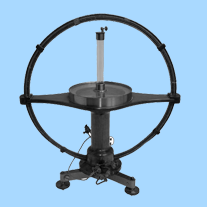
\includegraphics[valign=c, scale=0.23]{../materials/unfamiliar/1.png} & 1 & \makecell[l]{elektrische Spannung, prüfen\\{[electric current, measuring]}} & \makecell[l]{Makkaroni, formen\\{[macaroni, forming]}}\\
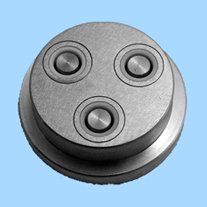
\includegraphics[valign=c, scale=0.23]{../materials/unfamiliar/2.png} & 2 & \makecell[l]{Makkaroni, formen\\{[macaroni, forming]}} & \makecell[l]{Kuh, vom Zaun abhalten\\{[cow, keeping away from the fence]}}\\
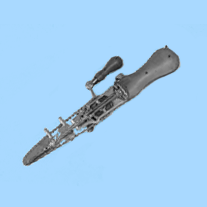
\includegraphics[valign=c, scale=0.23]{../materials/unfamiliar/3.png} & 3 & \makecell[l]{Knochen, sägen\\{[bones, sawing]}} & \makecell[l]{Streckenmaß, Sonnenlicht nutzen\\{[distance measure, using sunrays]}}\\
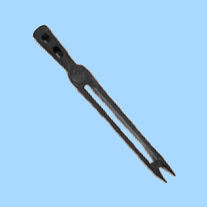
\includegraphics[valign=c, scale=0.23]{../materials/unfamiliar/4.png} & 4 & \makecell[l]{Unkraut, jäten\\{[weed, removing]}} & \makecell[l]{Uhr, mit Wärme betreiben\\{[clock, operating with heat]}}\\
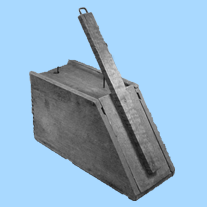
\includegraphics[valign=c, scale=0.23]{../materials/unfamiliar/5.png} & 5 & \makecell[l]{Mausefalle, zuschnappen\\{[mousetrap, snap-shutting]}} & \makecell[l]{Brillenglas, zuschneiden\\{[eyeglass lense, cutting]}}\\
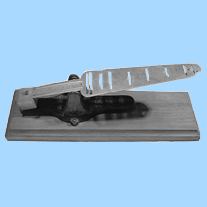
\includegraphics[valign=c, scale=0.23]{../materials/unfamiliar/6.png} & 6 & \makecell[l]{Goldmünzen, wiegen\\{[gold coin, weighing]}} & \makecell[l]{Farbe, vom Fenster abschleifen\\{[paint, scraping off the window]}}\\
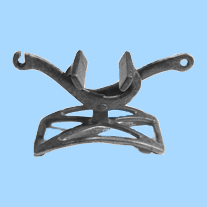
\includegraphics[valign=c, scale=0.23]{../materials/unfamiliar/7.png} & 7 & \makecell[l]{Knie, fixieren\\{[knee, fixating]}} & \makecell[l]{Buchstaben, tippen\\{[letter, typing]}}\\
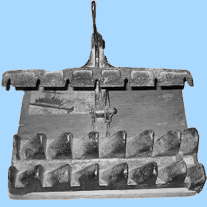
\includegraphics[valign=c, scale=0.23]{../materials/unfamiliar/8.png} & 8 & \makecell[l]{Eierkarton, pressen\\{[egg carton, pressing]}} & \makecell[l]{Tabak, zermahlen\\{[tobacco, pulverize]}}\\
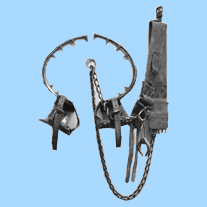
\includegraphics[valign=c, scale=0.23]{../materials/unfamiliar/9.png} & 9 & \makecell[l]{Baum, erklettern\\{[tree, climbing]}} & \makecell[l]{Rotation, Ladung erzeugen\\{[rotation, creating electric charge]}}\\
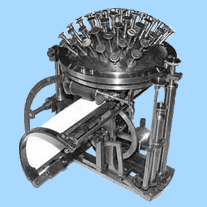
\includegraphics[valign=c, scale=0.23]{../materials/unfamiliar/10.png} & 10 & \makecell[l]{Buchstaben, tippen\\{[letter, typing]}} & \makecell[l]{Pferdehuf, Halt geben\\{[horse hoof, giving grip]}}\\
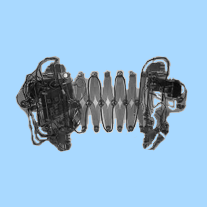
\includegraphics[valign=c, scale=0.23]{../materials/unfamiliar/11.png} & 11 & \makecell[l]{Akkordeon, spielen\\{[accordion, playing]}} & \makecell[l]{Seil, schneiden\\{[rope, cutting]}}\\
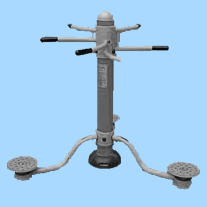
\includegraphics[valign=c, scale=0.23]{../materials/unfamiliar/12.png} & 12 & \makecell[l]{Körper, trainieren\\{[body, training]}} & \makecell[l]{Buch, offen halten\\{[book, binding]}}\\
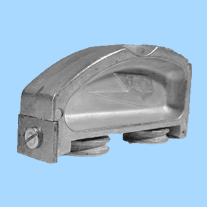
\includegraphics[valign=c, scale=0.23]{../materials/unfamiliar/13.png} & 13 & \makecell[l]{Farbe, vom Fenster abschleifen\\{[paint, scraping off the window]}} & \makecell[l]{von Hand, zentrifugieren\\{[by hand, centrifugating]}}\\
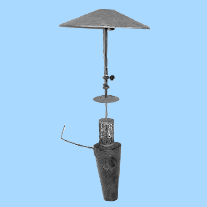
\includegraphics[valign=c, scale=0.23]{../materials/unfamiliar/14.png} & 14 & \makecell[l]{Außenbereich, heizen\\{[outdoor area, heating]}} & \makecell[l]{Rasierklinge, schärfen\\{[razor blade, sharpening]}}\\
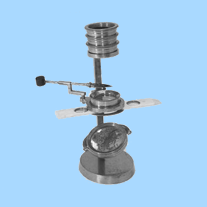
\includegraphics[valign=c, scale=0.23]{../materials/unfamiliar/15.png} & 15 & \makecell[l]{Pflanzenteile, vergrößern\\{[plant parts, magnifying]}} & \makecell[l]{Katzenklo, sich selbst reinigen\\{[litter box, self-cleaning]}}\\

\includegraphics[valign=c, scale=0.23]{../materials/unfamiliar/16.png} & 16 & \makecell[l]{Krawatten, aufhängen\\{[necktie, hanging up]}} & \makecell[l]{Zeichnungen, vermessen\\{[drawings, measuring]}}\\
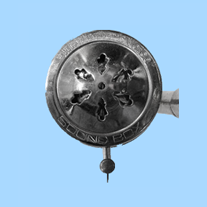
\includegraphics[valign=c, scale=0.23]{../materials/unfamiliar/17.png} & 17 & \makecell[l]{Schallplatte, abtasten\\{[vinyl record, reading]}} & \makecell[l]{Ball, katapultieren\\{[ball, catapulting]}}\\
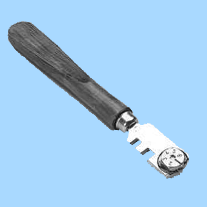
\includegraphics[valign=c, scale=0.23]{../materials/unfamiliar/18.png} & 18 & \makecell[l]{Glas, schneiden\\{[glass, cutting]}} & \makecell[l]{Eier, wiegen\\{[eggs, weighing]}}\\
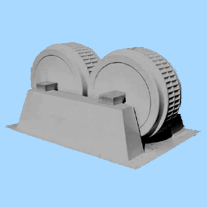
\includegraphics[valign=c, scale=0.23]{../materials/unfamiliar/19.png} & 19 & \makecell[l]{Briketts, pressen\\{[briquette, pressing]}} & \makecell[l]{Narkosemittel, abgeben\\{[anesthetic, administering]}}\\
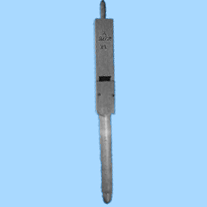
\includegraphics[valign=c, scale=0.23]{../materials/unfamiliar/20.png} & 20 & \makecell[l]{Orgelton, erzeugen\\{[organ sound, making]}} & \makecell[l]{Bandage, rollen\\{[bandage, rolling]}}\\
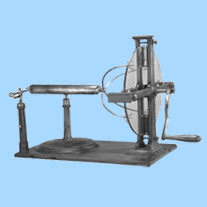
\includegraphics[valign=c, scale=0.23]{../materials/unfamiliar/21.png} & 21 & \makecell[l]{Spannung, erzeugen\\{[electric current, making]}} & \makecell[l]{Fußstütze, reiten\\{[footrest, horseback riding]}}\\
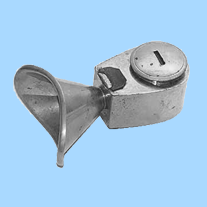
\includegraphics[valign=c, scale=0.23]{../materials/unfamiliar/22.png} & 22 & \makecell[l]{Narkosemittel, abgeben\\{[anesthetic, administering]}} & \makecell[l]{Nüsse, aufbrechen\\{[nuts, cracking]}}\\
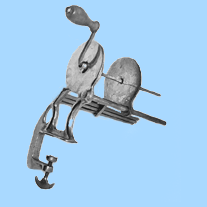
\includegraphics[valign=c, scale=0.23]{../materials/unfamiliar/23.png} & 23 & \makecell[l]{Bandage, rollen\\{[bandage, rolling]}} & \makecell[l]{Schnee, rodeln\\{[snow, sleighing]}}\\
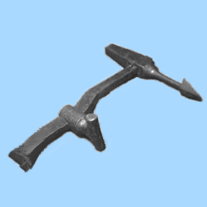
\includegraphics[valign=c, scale=0.23]{../materials/unfamiliar/24.png} & 24 & \makecell[l]{Weinfass, Loch einschlagen\\{[wine barrel, smashing a hole]}} & \makecell[l]{Tier, einfangen\\{[animal, trapping]}}\\
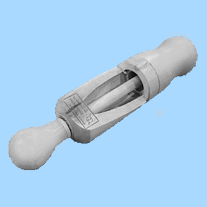
\includegraphics[valign=c, scale=0.23]{../materials/unfamiliar/25.png} & 25 & \makecell[l]{Flaschenkorken, einführen\\{[bottle cork, inserting]}} & \makecell[l]{Pferd, im Moor laufen\\{[horse, walking in the moor]}}\\
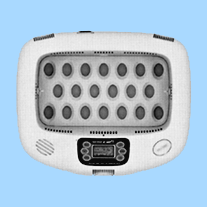
\includegraphics[valign=c, scale=0.23]{../materials/unfamiliar/26.png} & 26 & \makecell[l]{Automat, Eier ausbrüten\\{[machine, incubating eggs]}} & \makecell[l]{Windgeschwindigkeit, messen\\{[wind speed, measuring]}}\\
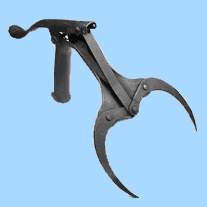
\includegraphics[valign=c, scale=0.23]{../materials/unfamiliar/27.png} & 27 & \makecell[l]{Korngarbe, greifen\\{[sheaf, grabbing]}} & \makecell[l]{Treibhaus, heizen\\{[glass house, heating]}}\\
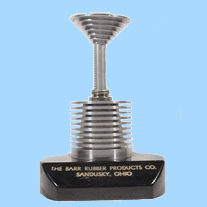
\includegraphics[valign=c, scale=0.23]{../materials/unfamiliar/28.png} & 28 & \makecell[l]{Brief, wiegen\\{[letter, weighing]}} & \makecell[l]{Korngarbe, greifen\\{[sheaf, grabbing]}}\\
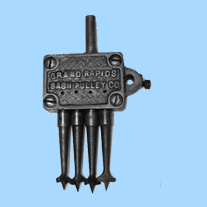
\includegraphics[valign=c, scale=0.23]{../materials/unfamiliar/29.png} & 29 & \makecell[l]{Löcher, bohren\\{[hole, drilling]}} & \makecell[l]{Sonnenlicht, Intensität messen\\{[sunlight, measure intensity]}}\\
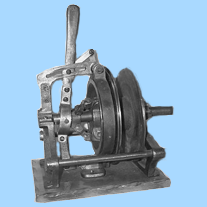
\includegraphics[valign=c, scale=0.23]{../materials/unfamiliar/30.png} & 30 & \makecell[l]{Angelschnur, kurbeln\\{[fishing line, winding]}} & \makecell[l]{Glaskörper, musizieren\\{[glass body, making music]}}\\
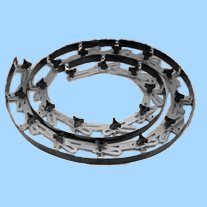
\includegraphics[valign=c, scale=0.23]{../materials/unfamiliar/31.png} & 31 & \makecell[l]{Kurven, malen\\{[curve, drawing]}} & \makecell[l]{Nussöl, pressen\\{[nut oil, pressing]}}\\
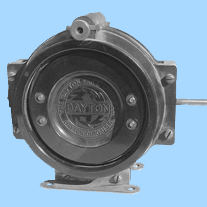
\includegraphics[valign=c, scale=0.23]{../materials/unfamiliar/32.png} & 32 & \makecell[l]{Radiofrequenz, einstellen\\{[radio frequency, tuning]}} & \makecell[l]{Erektion, helfen\\{[erection, helping]}}\\
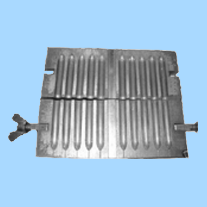
\includegraphics[valign=c, scale=0.23]{../materials/unfamiliar/33.png} & 33 & \makecell[l]{Zäpfchen, pressen\\{[suppository, pressing]}} & \makecell[l]{Unkraut, jäten\\{[weed, removing]}}\\
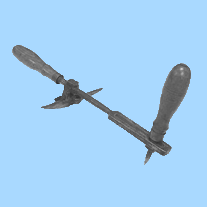
\includegraphics[valign=c, scale=0.23]{../materials/unfamiliar/34.png} & 34 & \makecell[l]{Fass, öffnen\\{[barrel, opening]}} & \makecell[l]{Pflanzenteile, vergrößern\\{[plant parts, magnifying]}}\\
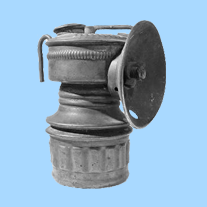
\includegraphics[valign=c, scale=0.23]{../materials/unfamiliar/35.png} & 35 & \makecell[l]{Bergbaustollen, beleuchten\\{[mining tunnel, lightening]}} & \makecell[l]{Knie, fixieren\\{[knee, fixating]}}\\
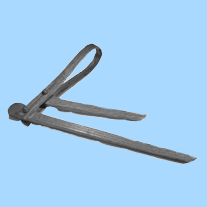
\includegraphics[valign=c, scale=0.23]{../materials/unfamiliar/36.png} & 36 & \makecell[l]{Kuh, vom Zaun abhalten\\{[cow, keeping away from the fence]}} & \makecell[l]{Radiofrequenz, einstellen\\{[radio frequency, tuning]}}\\
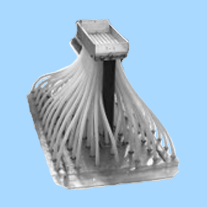
\includegraphics[valign=c, scale=0.23]{../materials/unfamiliar/37.png} & 37 & \makecell[l]{Saatgut, gleichmäßig aussäen\\{[seeds, sowing evenly]}} & \makecell[l]{Fass, öffnen\\{[barrel, opening]}}\\
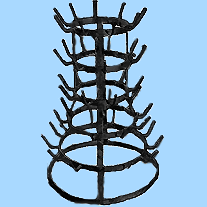
\includegraphics[valign=c, scale=0.23]{../materials/unfamiliar/38.png} & 38 & \makecell[l]{Flaschen, trocknen\\{[bottles, drying]}} & \makecell[l]{Bleistift, anspitzen\\{[pencil, sharpening]}}\\
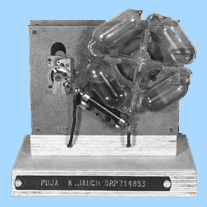
\includegraphics[valign=c, scale=0.23]{../materials/unfamiliar/39.png} & 39 & \makecell[l]{Uhr, mit Wärme betreiben\\{[clock, operating with heat]}} & \makecell[l]{Körper, untersuchen\\{[body, training]}}\\
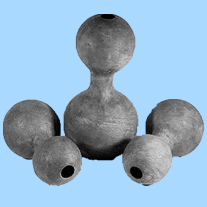
\includegraphics[valign=c, scale=0.23]{../materials/unfamiliar/40.png} & 40 & \makecell[l]{Tonpott, trommeln\\{[clay pot, drumming]}} & \makecell[l]{Piano, stimmen\\{[piano, tuning]}}\\
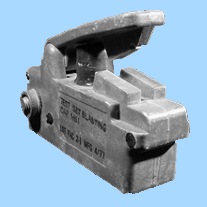
\includegraphics[valign=c, scale=0.23]{../materials/unfamiliar/41.png} & 41 & \makecell[l]{Sprengstoffexplosion, auslösen\\{[dynamite explosion, triggering]}} & \makecell[l]{Fisch, wiegen\\{[fish, weighing]}}\\
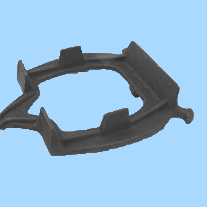
\includegraphics[valign=c, scale=0.23]{../materials/unfamiliar/42.png} & 42 & \makecell[l]{Pferdehuf, Halt geben\\{[horse hoof, giving grip]}} & \makecell[l]{Zäpfchen, pressen\\{[suppository, pressing]}}\\
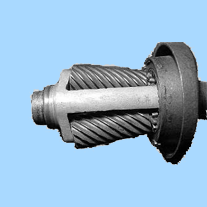
\includegraphics[valign=c, scale=0.23]{../materials/unfamiliar/43.png} & 43 & \makecell[l]{Bleistift, anspitzen\\{[pencil, sharpening]}} & \makecell[l]{Angel, Köder markieren\\{[fishing rod, marking bait]}}\\
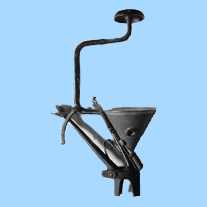
\includegraphics[valign=c, scale=0.23]{../materials/unfamiliar/44.png} & 44 & \makecell[l]{Nussöl, pressen\\{[nut oil, pressing]}} & \makecell[l]{Zeichen, einbrennen\\{[marks, burning in]}}\\
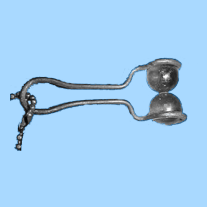
\includegraphics[valign=c, scale=0.23]{../materials/unfamiliar/45.png} & 45 & \makecell[l]{Rasierklinge, schärfen\\{[razor blade, sharpening]}} & \makecell[l]{Kurven, malen\\{[curve, drawing]}}\\
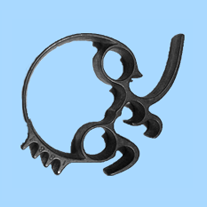
\includegraphics[valign=c, scale=0.23]{../materials/unfamiliar/46.png} & 46 & \makecell[l]{heiße Platten, anheben\\{[hot plates, lifting]}} & \makecell[l]{Kleidung, im Eimer waschen\\{[clothes, washing in a bucket]}}\\
\includegraphics[valign=c, scale=0.23]{../materials/unfamiliar/47.png} & 47 & \makecell[l]{Film, aufspulen\\{[film roll, winding]}} & \makecell[l]{Mund, offen halten\\{[mouth, keeping open]}}\\
\includegraphics[valign=c, scale=0.23]{../materials/unfamiliar/48.png} & 48 & \makecell[l]{Waffe, entflammen\\{[weapon, inflaming]}} & \makecell[l]{Uhrzeit, anzeigen\\{[time, displaying]}}\\
\includegraphics[valign=c, scale=0.23]{../materials/unfamiliar/49.png} & 49 & \makecell[l]{Mikroskop-Proben, schneiden\\{[microscopic samples, slicing]}} & \makecell[l]{heiße Platten, anheben\\{[hot plates, lifting]}}\\
\includegraphics[valign=c, scale=0.23]{../materials/unfamiliar/50.png} & 50 & \makecell[l]{Glaskörper, musizieren\\{[glass body, making music]}} & \makecell[l]{Kork, flach pressen\\{[cork, pressing flat]}}\\
\includegraphics[valign=c, scale=0.23]{../materials/unfamiliar/51.png} & 51 & \makecell[l]{Dampf, zerstäuben\\{[steam, spraying]}} & \makecell[l]{Buch, binden\\{[book, opening]}}\\
\includegraphics[valign=c, scale=0.23]{../materials/unfamiliar/52.png} & 52 & \makecell[l]{Mandeln, operieren\\{[kidneys, operating]}} & \makecell[l]{Film, aufspulen\\{[film roll, winding]}}\\
\includegraphics[valign=c, scale=0.23]{../materials/unfamiliar/53.png} & 53 & \makecell[l]{Toastbrot, rösten\\{[toast, roasting]}} & \makecell[l]{Autobatterie, Spannung testen\\{[car battery, measuring voltage]}}\\
\includegraphics[valign=c, scale=0.23]{../materials/unfamiliar/54.png} & 54 & \makecell[l]{Fußstütze, reiten\\{[footrest, horseback riding]}} & \makecell[l]{Stromstärke, messen\\{[current, measuring]}}\\
\includegraphics[valign=c, scale=0.23]{../materials/unfamiliar/55.png} & 55 & \makecell[l]{Türgelenk, Feuer überstehen\\{[door hinge, survining fires]}} & \makecell[l]{Botschaft, telegrafieren\\{[message, telegraphing]}}\\
\includegraphics[valign=c, scale=0.23]{../materials/unfamiliar/56.png} & 56 & \makecell[l]{Schnee, rodeln\\{[snow, sleighing]}} & \makecell[l]{Dampf, zerstäuben\\{[steam, spraying]}}\\
\includegraphics[valign=c, scale=0.23]{../materials/unfamiliar/57.png} & 57 & \makecell[l]{Nüsse, aufbrechen\\{[nuts, cracking]}} & \makecell[l]{Ziegelsteine, formen\\{[bricks, forming]}}\\
\includegraphics[valign=c, scale=0.23]{../materials/unfamiliar/58.png} & 58 & \makecell[l]{Radiergummi, mit Strom betreiben\\{[eraser, operating with electricity]}} & \makecell[l]{Münzen, aufbewahren\\{[coins, storing]}}\\
\includegraphics[valign=c, scale=0.23]{../materials/unfamiliar/59.png} & 59 & \makecell[l]{Treibhaus, heizen\\{[glass house, heating]}} & \makecell[l]{Messer, schleifen\\{[knife, sharpening]}}\\
\includegraphics[valign=c, scale=0.23]{../materials/unfamiliar/60.png} & 60 & \makecell[l]{Botschaft, telegrafieren\\{[message, telegraphing]}} & \makecell[l]{Toastbrot, rösten\\{[toast, roasting]}}\\
\includegraphics[valign=c, scale=0.23]{../materials/unfamiliar/61.png} & 61 & \makecell[l]{Angel, Köder markieren\\{[fishing rod, marking bait]}} & \makecell[l]{Baum, erklettern\\{[tree, climbing]}}\\
\includegraphics[valign=c, scale=0.23]{../materials/unfamiliar/62.png} & 62 & \makecell[l]{Katzenklo, sich selbst reinigen\\{[litter box, self-cleaning]}} & \makecell[l]{Tankfüllstand, messen\\{[fuel tank level, gauging]}}\\
\includegraphics[valign=c, scale=0.23]{../materials/unfamiliar/63.png} & 63 & \makecell[l]{Körper, untersuchen\\{[body, examining]}} & \makecell[l]{Schuhe, auf Eis laufen\\{[shoes, walking on ice]}}\\
\includegraphics[valign=c, scale=0.23]{../materials/unfamiliar/64.png} & 64 & \makecell[l]{Brillenglas, zuschneiden\\{[eyeglass lense, cutting]}} & \makecell[l]{Saatgut, gleichmäßig aussäen\\{[seeds, sowing evenly]}}\\
\includegraphics[valign=c, scale=0.23]{../materials/unfamiliar/65.png} & 65 & \makecell[l]{Draht, wickeln\\{[wire, winding]}} & \makecell[l]{Bergbaustollen, beleuchten\\{[mining tunnel, lightening]}}\\
\includegraphics[valign=c, scale=0.23]{../materials/unfamiliar/66.png} & 66 & \makecell[l]{Buch, offen halten\\{[book, opening]}} & \makecell[l]{Sprengstoffexplosion, auslösen\\{[dynamite explosion, triggering]}}\\
\includegraphics[valign=c, scale=0.23]{../materials/unfamiliar/67.png} & 67 & \makecell[l]{Feldanbau, häckseln\\{[harvest, chopping]}} & \makecell[l]{Draht, wickeln\\{[wire, winding]}}\\
\includegraphics[valign=c, scale=0.23]{../materials/unfamiliar/68.png} & 68 & \makecell[l]{Schnurlot, absenken\\{[plummet, letting down]}} & \makecell[l]{Korken, formen\\{[bottle cork, forming]}}\\
\includegraphics[valign=c, scale=0.23]{../materials/unfamiliar/69.png} & 69 & \makecell[l]{Sternenbilder, vermessen\\{[stellar constellation, measuring]}} & \makecell[l]{Schnurlot, absenken\\{[plummet, letting down]}}\\
\includegraphics[valign=c, scale=0.23]{../materials/unfamiliar/70.png} & 70 & \makecell[l]{Nachricht, morsen\\{[message, signalling]}} & \makecell[l]{Feldanbau, häckseln\\{[harvest, chopping]}}\\
\includegraphics[valign=c, scale=0.23]{../materials/unfamiliar/71.png} & 71 & \makecell[l]{Musikgerät, stampfen\\{[musical instrument, stamping]}} & \makecell[l]{Goldmünzen, wiegen\\{[gold coin, weighing]}}\\
\includegraphics[valign=c, scale=0.23]{../materials/unfamiliar/72.png} & 72 & \makecell[l]{Schuhe, auf Eis laufen\\{[shoes, walking on ice]}} & \makecell[l]{Geschwindigkeit, ermitteln\\{[speed, determining]}}\\
\includegraphics[valign=c, scale=0.23]{../materials/unfamiliar/73.png} & 73 & \makecell[l]{Geschwindigkeit, ermitteln\\{[speed, determining]}} & \makecell[l]{Mausefalle, zuschnappen\\{[mousetrap, snap-shutting]}}\\
\includegraphics[valign=c, scale=0.23]{../materials/unfamiliar/74.png} & 74 & \makecell[l]{Zeichen, einbrennen\\{[marks, burning in]}} & \makecell[l]{Luftdruck, messen\\{[air pressure, measuring]}}\\
\includegraphics[valign=c, scale=0.23]{../materials/unfamiliar/75.png} & 75 & \makecell[l]{Tabak, zermahlen\\{[tobacco, pulverize]}} & \makecell[l]{Flaschen, trocknen\\{[bottles, drying]}}\\
\includegraphics[valign=c, scale=0.23]{../materials/unfamiliar/76.png} & 76 & \makecell[l]{Stromstärke, messen\\{[current, measuring]}} & \makecell[l]{Mandeln, operieren\\{[kidneys, operating]}}\\
\includegraphics[valign=c, scale=0.23]{../materials/unfamiliar/77.png} & 77 & \makecell[l]{Tier, einfangen\\{[animal, trapping]}} & \makecell[l]{Maiskolben, entkörnen\\{[corncob, removing grains]}}\\
\includegraphics[valign=c, scale=0.23]{../materials/unfamiliar/78.png} & 78 & \makecell[l]{Messer, schleifen\\{[knife, sharpening]}} & \makecell[l]{Schritte, vergrößern\\{[steps, extending]}}\\
\includegraphics[valign=c, scale=0.23]{../materials/unfamiliar/79.png} & 79 & \makecell[l]{Leierkasten, klingen\\{[barrel organ, making sounds]}} & \makecell[l]{Fass, anheben\\{[barrel, lifting]}}\\
\includegraphics[valign=c, scale=0.23]{../materials/unfamiliar/80.png} & 80 & \makecell[l]{Buch, binden\\{[book, binding]}} & \makecell[l]{Löcher, bohren\\{[hole, drilling]}}\\
\includegraphics[valign=c, scale=0.23]{../materials/unfamiliar/81.png} & 81 & \makecell[l]{Kork, flach pressen\\{[cork, pressing flat]}} & \makecell[l]{Elektroschock, spielen\\{[electric shock, playing]}}\\
\includegraphics[valign=c, scale=0.23]{../materials/unfamiliar/82.png} & 82 & \makecell[l]{Tabletten, zerteilen\\{[pill, splitting]}} & \makecell[l]{Blumentopf, sich selbst wässern\\{[flower pot, self-watering]}}\\
\includegraphics[valign=c, scale=0.23]{../materials/unfamiliar/83.png} & 83 & \makecell[l]{Fass, anheben\\{[barrel, lifting]}} & \makecell[l]{Mikroskop-Proben, schneiden\\{[microscopic samples, slicing]}}\\
\includegraphics[valign=c, scale=0.23]{../materials/unfamiliar/84.png} & 84 & \makecell[l]{Pferd, im Moor laufen\\{[horse, walking in the moor]}} & \makecell[l]{Luft, abpumpen\\{[air, pumping out]}}\\
\includegraphics[valign=c, scale=0.23]{../materials/unfamiliar/85.png} & 85 & \makecell[l]{altes Ritual, hacken\\{[ancient ritual, chopping]}} & \makecell[l]{Spannung, erzeugen\\{[electric current, making]}}\\
\includegraphics[valign=c, scale=0.23]{../materials/unfamiliar/86.png} & 86 & \makecell[l]{Kleidung, im Eimer waschen\\{[clothes, washing in a bucket]}} & \makecell[l]{Türgelenk, Feuer überstehen\\{[door hinge, survining fires]}}\\
\includegraphics[valign=c, scale=0.23]{../materials/unfamiliar/87.png} & 87 & \makecell[l]{Maiskolben, entkörnen\\{[corncob, removing grains]}} & \makecell[l]{Brief, wiegen\\{[letter, weighing]}}\\
\includegraphics[valign=c, scale=0.23]{../materials/unfamiliar/88.png} & 88 & \makecell[l]{Ball, katapultieren\\{[ball, catapulting]}} & \makecell[l]{Radiergummi, mit Strom betreiben\\{[eraser, operating with electricity]}}\\
\includegraphics[valign=c, scale=0.23]{../materials/unfamiliar/89.png} & 89 & \makecell[l]{Zeichnungen, vermessen\\{[drawings, measuring]}} & \makecell[l]{Brenner, löten\\{[burner, soldering]}}\\
\includegraphics[valign=c, scale=0.23]{../materials/unfamiliar/90.png} & 90 & \makecell[l]{Elektroschock, spielen\\{[electric shock, playing]}} & \makecell[l]{Weinfass, Loch einschlagen\\{[wine barrel, smashing a hole]}}\\
\includegraphics[valign=c, scale=0.23]{../materials/unfamiliar/91.png} & 91 & \makecell[l]{Lieferungen, abzählen\\{[deliveries, counting]}} & \makecell[l]{Außenbereich, heizen\\{[outdoor area, heating]}}\\
\includegraphics[valign=c, scale=0.23]{../materials/unfamiliar/92.png} & 92 & \makecell[l]{Rotation, Ladung erzeugen\\{[rotation, creating electric charge]}} & \makecell[l]{Musikgerät, stampfen\\{[musical instrument, stamping]}}\\
\includegraphics[valign=c, scale=0.23]{../materials/unfamiliar/93.png} & 93 & \makecell[l]{Herz, durch Maschine ersetzen\\{[heart, replacing with machine]}} & \makecell[l]{Kerzen, löschen\\{[candles, extinguishing]}}\\
\includegraphics[valign=c, scale=0.23]{../materials/unfamiliar/94.png} & 94 & \makecell[l]{Seil, schneiden\\{[rope, cutting]}} & \makecell[l]{Akkordeon, spielen\\{[accordion, playing]}}\\
\includegraphics[valign=c, scale=0.23]{../materials/unfamiliar/95.png} & 95 & \makecell[l]{Fisch, wiegen\\{[fish, weighing]}} & \makecell[l]{Herz, durch Maschine ersetzen\\{[heart, replacing with machine]}}\\
\includegraphics[valign=c, scale=0.23]{../materials/unfamiliar/96.png} & 96 & \makecell[l]{Kerzen, löschen\\{[candles, extinguishing]}} & \makecell[l]{Körper, trainieren\\{[body, examining]}}\\
\includegraphics[valign=c, scale=0.23]{../materials/unfamiliar/97.png} & 97 & \makecell[l]{Korken, formen\\{[bottle cork, forming]}} & \makecell[l]{Sternenbilder, vermessen\\{[stellar constellation, measuring]}}\\
\includegraphics[valign=c, scale=0.23]{../materials/unfamiliar/98.png} & 98 & \makecell[l]{Erektion, helfen\\{[erection, helping]}} & \makecell[l]{Waffe, werfen\\{[weapn, throwing]}}\\
\includegraphics[valign=c, scale=0.23]{../materials/unfamiliar/99.png} & 99 & \makecell[l]{Streckenmaß, Sonnenlicht nutzen\\{[distance measure, using sunrays]}} & \makecell[l]{Kartoffeln, stampfen\\{[potatoes, mashing]}}\\
\includegraphics[valign=c, scale=0.23]{../materials/unfamiliar/100.png} & 100 & \makecell[l]{Luftdruck, messen\\{[air pressure, measuring]}} & \makecell[l]{Knochen, sägen\\{[bones, sawing]}}\\
\includegraphics[valign=c, scale=0.23]{../materials/unfamiliar/101.png} & 101 & \makecell[l]{Piano, stimmen\\{[piano, tuning]}} & \makecell[l]{Eierkarton, pressen\\{[egg carton, pressing]}}\\
\includegraphics[valign=c, scale=0.23]{../materials/unfamiliar/102.png} & 102 & \makecell[l]{von Hand, zentrifugieren\\{[by hand, centrifugating]}} & \makecell[l]{Lieferungen, abzählen\\{[deliveries, counting]}}\\
\includegraphics[valign=c, scale=0.23]{../materials/unfamiliar/103.png} & 103 & \makecell[l]{Kartoffeln, stampfen\\{[potatoes, mashing]}} & \makecell[l]{Nachricht, morsen\\{[message, signalling]}}\\
\includegraphics[valign=c, scale=0.23]{../materials/unfamiliar/104.png} & 104 & \makecell[l]{Waffe, werfen\\{[weapn, throwing]}} & \makecell[l]{elektrische Spannung, prüfen\\{[electric current, measuring]}}\\
\includegraphics[valign=c, scale=0.23]{../materials/unfamiliar/105.png} & 105 & \makecell[l]{Tankfüllstand, messen\\{[fuel tank level, gauging]}} & \makecell[l]{Tonpott, trommeln\\{[clay pot, drumming]}}\\
\includegraphics[valign=c, scale=0.23]{../materials/unfamiliar/106.png} & 106 & \makecell[l]{Uhrzeit, anzeigen\\{[time, displaying]}} & \makecell[l]{altes Ritual, hacken\\{[ancient ritual, chopping]}}\\
\includegraphics[valign=c, scale=0.23]{../materials/unfamiliar/107.png} & 107 & \makecell[l]{Windgeschwindigkeit, messen\\{[wind speed, measuring]}} & \makecell[l]{Waffe, entflammen\\{[weapon, inflaming]}}\\
\includegraphics[valign=c, scale=0.23]{../materials/unfamiliar/108.png} & 108 & \makecell[l]{Schlüsselloch, stanzen\\{[keyhole, punching]}} & \makecell[l]{Automat, Eier ausbrüten\\{[machine, incubating eggs]}}\\
\includegraphics[valign=c, scale=0.23]{../materials/unfamiliar/109.png} & 109 & \makecell[l]{Ziegelsteine, formen\\{[bricks, forming]}} & \makecell[l]{Schallplatte, abtasten\\{[vinyl record, reading]}}\\
\includegraphics[valign=c, scale=0.23]{../materials/unfamiliar/110.png} & 110 & \makecell[l]{Becher, Schall auffangen\\{[drinking cup, picking up sound]}} & \makecell[l]{Schlüsselloch, stanzen\\{[keyhole, punching]}}\\
\includegraphics[valign=c, scale=0.23]{../materials/unfamiliar/111.png} & 111 & \makecell[l]{Luft, abpumpen\\{[air, pumping out]}} & \makecell[l]{Briketts, pressen\\{[briquette, pressing]}}\\
\includegraphics[valign=c, scale=0.23]{../materials/unfamiliar/112.png} & 112 & \makecell[l]{Mund, offen halten\\{[mouth, keeping open]}} & \makecell[l]{Orgelton, erzeugen\\{[organ sound, making]}}\\
\includegraphics[valign=c, scale=0.23]{../materials/unfamiliar/113.png} & 113 & \makecell[l]{Autobatterie, Spannung testen\\{[car battery, measuring voltage]}} & \makecell[l]{Becher, Schall auffangen\\{[drinking cup, picking up sound]}}\\
\includegraphics[valign=c, scale=0.23]{../materials/unfamiliar/114.png} & 114 & \makecell[l]{Sonnenlicht, Intensität messen\\{[sunlight, measure intensity]}} & \makecell[l]{Krawatten, aufhängen\\{[necktie, hanging up]}}\\
\includegraphics[valign=c, scale=0.23]{../materials/unfamiliar/115.png} & 115 & \makecell[l]{Kutschrad, anschließen\\{[carriage wheel, locking]}} & \makecell[l]{Angelschnur, kurbeln\\{[fishing line, winding]}}\\
\includegraphics[valign=c, scale=0.23]{../materials/unfamiliar/116.png} & 116 & \makecell[l]{Eier, wiegen\\{[eggs, weighing]}} & \makecell[l]{Leierkasten, klingen\\{[barrel organ, making sounds]}}\\
\includegraphics[valign=c, scale=0.23]{../materials/unfamiliar/117.png} & 117 & \makecell[l]{Blumentopf, sich selbst wässern\\{[flower pot, self-watering]}} & \makecell[l]{Glas, schneiden\\{[glass, cutting]}}\\
\includegraphics[valign=c, scale=0.23]{../materials/unfamiliar/118.png} & 118 & \makecell[l]{Schritte, vergrößern\\{[steps, extending]}} & \makecell[l]{Tabletten, zerteilen\\{[pill, splitting]}}\\
\includegraphics[valign=c, scale=0.23]{../materials/unfamiliar/119.png} & 119 & \makecell[l]{Münzen, aufbewahren\\{[coins, storing]}} & \makecell[l]{Kutschrad, anschließen\\{[carriage wheel, locking]}}\\
\includegraphics[valign=c, scale=0.23]{../materials/unfamiliar/120.png} & 120 & \makecell[l]{Brenner, löten\\{[burner, soldering]}} & \makecell[l]{Flaschenkorken einführen, einführen\\{[bottle cork, inserting]}}\\
\bottomrule
\end{longtable}

}

\end{ThreePartTable}
\end{center}

\newpage

\hypertarget{appendix-b-linear-mixed-effects-models}{%
\subsection*{Appendix B: Linear Mixed-Effects Models}\label{appendix-b-linear-mixed-effects-models}}
\addcontentsline{toc}{subsection}{Appendix B: Linear Mixed-Effects Models}

\noindent Linear mixed-effects models after model selection for Experiment 1:

\footnotesize

\begin{verbatim}
## P1 ~ 1 + part + condition + part:condition + (1 + part | participant)
## N170 ~ 1 + part + condition + part:condition + (1 + part + condition | participant)
## N400 ~ 1 + part + condition + part:condition + (1 + part + condition | participant)
\end{verbatim}

\normalsize

\noindent Linear mixed-effects models after model selection for Experiment 2:

\footnotesize

\begin{verbatim}
## P1 ~ 1 + part + condition + part:condition + (1 | participant)
## N170 ~ 1 + part + condition + part:condition + (1 + part | participant)
## N400 ~ 1 + part + condition + part:condition + (1 + part | participant)
\end{verbatim}

\normalsize

\noindent Linear mixed-effects models after model selection for Experiments 1 and 2 combined:

\footnotesize

\begin{verbatim}
## P1 ~ 1 + part + condition + part:condition + experiment + part:experiment + 
##     condition:experiment + part:condition:experiment + (1 + part | participant)
## N170 ~ 1 + part + condition + part:condition + experiment + part:experiment + 
##     condition:experiment + part:condition:experiment + (1 + part + condition | 
##     participant)
## N400 ~ 1 + part + condition + part:condition + experiment + part:experiment + 
##     condition:experiment + part:condition:experiment + (1 + part | participant)
\end{verbatim}

\normalsize

\newpage
\setlength{\parindent}{0.5in}

\hypertarget{declaration-of-authorship}{%
\section*{Declaration of Authorship}\label{declaration-of-authorship}}
\addcontentsline{toc}{section}{Declaration of Authorship}

I hereby declare that the present thesis has not been submitted as a part of any other examination procedure and has been independently written. All passages, including those from the internet, which were used directly or in modified form, especially those sources using text, graphs, charts or pictures, are indicated as such. I realize that an infringement of these principles which would amount to either an attempt of deception or deceit will lead to the institution of proceedings against myself.

\vspace*{20mm}

\noindent
Alexander Enge\newline
Berlin, 26.01.2021

\clearpage

\mbox{}\thispagestyle{empty}\clearpage

\clearpage

\mbox{}\thispagestyle{empty}\clearpage


\end{document}
